\documentclass[12pt, a4paper, oneside, onecolumn]{article}
\usepackage[left=3cm,top=3cm,right=2cm,bottom=2cm]{geometry}
\usepackage[brazilian]{babel}
\usepackage[utf8]{inputenc}
\usepackage{indentfirst}
\setlength\parindent{1.5cm}
\usepackage{amsmath}
\usepackage{graphicx}
\usepackage{fancyhdr}
\fancyhead{}
\fancyfoot{}
\rhead{\thepage}
\renewcommand{\headrulewidth}{0pt}
\pagestyle{fancy}
\usepackage{tocloft}
\usepackage{array}
\usepackage{makecell}
%\usepackage{tabularx}

\usepackage[dvipsnames]{xcolor}

%no hyphenization
\tolerance=1
\emergencystretch=\maxdimen
\hyphenpenalty=10000
\hbadness=10000


%\usepackage{fontspec}
%\setmainfont{Arial}
\usepackage{lmodern}
\usepackage[T1]{fontenc}

\linespread{1.5}

\usepackage[colorlinks = true,
            linkcolor = black,
            urlcolor  = black,
            citecolor = blue,
            anchorcolor = yellow]{hyperref}

\usepackage[alf]{abntex2cite}
\usepackage{subfigure}

\usepackage[acronym]{glossaries}
\makeglossaries

\usepackage{enumitem}
\setlist{nosep}


\begin{document}

\begin{center}
    
    \begin{figure}[h!]
        \centering
        
\includegraphics[width=0.3\textwidth]{Outros/brasao_ufpe.png}
    \end{figure}    
    \textbf{
        \uppercase{
        Universidade Federal de Pernambuco \\
        Centro de Ciências Sociais Aplicadas \\
        Curso de Ciências Econômicas
        }
    }

    \vspace*{5cm}
    \uppercase{Paulo Francisco da Silva Júnior}
    \vspace*{3cm}
    
    \textbf{\uppercase{Impactos da Incerteza sobre a atividade econômica dos estados brasileiros}}
    
    \vspace*{\fill}
    \textbf{Recife \\ 2025}
    
    
\end{center}
\thispagestyle{empty}
\setcounter{page}{1}
\begin{center}
    \textbf{\uppercase{Paulo Francisco da Silva Júnior}}
    \vspace*{5cm}

    \textbf{\uppercase{Impactos da Incerteza sobre a atividade econômica dos estados brasileiros}}
    \vspace*{5cm}

    \begin{flushright}
        \begin{minipage}{.5\textwidth}
            Monografia apresentada ao Departamento de Ciências Econômicas, como exigência parcial para a obtenção do título de Bacharel em Ciências Econômicas, pela Universidade Federal de Pernambuco.
            \vspace*{0.7cm}
            \\
            \texwtbf{Orientador}: Prof. Dr. Marcelo Eduardo Alves da Silva 
        \end{minipage}
    \end{flushright}
    
    \vspace*{\fill}
    \textbf{Recife \\ 2025}
    
    
\end{center}
\thispagestyle{empty}
\begin{center}
    \textbf{\uppercase{Paulo Francisco da Silva Júnior}}
    \vspace*{1cm}

    \textbf{\uppercase{Impactos da Incerteza sobre a atividade econômica dos estados brasileiros}}
    \vspace*{1cm}

    \begin{flushright}
        \begin{minipage}{.5\textwidth}
            Monografia apresentada ao Departamento de Ciências Econômicas, como exigência parcial para a obtenção do título de Bacharel em Ciências Econômicas, pela Universidade Federal de Pernambuco.
            \vspace*{0.7cm}
        \end{minipage}
    \end{flushright}
    \vspace*{2cm}
    \begin{flushleft}
        Aprovado em: 10 de Abril de 2025 
        \newline
        Banca examinadora:
    \end{flushleft}
    

    \begin{flushright}
        \begin{minipage}{.8\textwidth}
            \vspace*{2cm}
            \hrule{}
            \vspace*{0.25cm}
            Prof. Dr. Marcelo Eduardo Alves da Silva \newline
            Departamento de Economia da UFPE

            \vspace*{2cm}
            \hrule{}
            \vspace*{0.25cm}
            Prof. Dr. André Matos Magalhães \newline
            Departamento de Economia da UFPE
        \end{minipage}
    \end{flushright}
    
    \vspace*{\fill}
    \textbf{Recife \\ 2025}
    
    
\end{center}
\thispagestyle{empty}
%\vspace*{\fill}
\begin{center}
    Eu dedico essa monografia aos meus pais () por sempre acreditarem em mim.
    \newline 
    Frase curta.
\end{center}
\vspace*{\fill}
\thispagestyle{empty}
\begin{center}
    \textbf{\uppercase{Agradecimentos}}
    \vspace{1cm}
\end{center}

Agradeço primeiramente a Deus por ter me dado sua graça e a oportunidade de participar dessa jornada acadêmica, juntamente com os demais desafios e projetos que vieram com ela. Destaco minha participação no Programa de Educação Tutorial (PET), como monitor das disciplinas de economia e apresentação de minicursos, no desenvolvimento de uma startup no programa Projetão CIn, no Programa Institucional de Bolsas de Iniciação Científica (PIBIC), na gincana regional e nacional de economia, no estágio no Banco Santander e na participação dos demais eventos.


À minha família, que sempre me forneceu apoio e a quem sou muito grato. Em especial, meus pais, Paulo e Selma, pelo suporte, compreensão e paciência diárias. 


Ao meu orientador, professor Marcelo Eduardo, por quem tenho admiração pessoal e profissional. Agradeço pela compreensão, paciência, conselhos e por acreditar no meu potencial. Agradeço também ao professor André Magalhães por todo o suporte e conselhos fornecidos. 


Aos amigos de faculdade que conheci nesta jornada, em especial, Caio Coutinho, Charles dos Santos, João Oscar, João Pedro Miranda e Thiago Henrique de França.


Aos amigos de trabalho do Santander que me proporcionaram uma vivência prática no mercado financeiro. Essencialmente, a equipe de riscos da rede nordeste: Camila de Santana, Dayvson de Melo, Fernando Vassalo e Waldyr Brissant.


As demais pessoas fora do âmbito profissional ou acadêmico que me apoiaram, principalmente aos amigos próximos: Almir Melo, Ellen Nunes e Thays Maria.

%Por último mas não menos importante, à minha princesa, Ellen Miranda, suportando minhas ligações sobre os papos chatos de \textit{economêz} durante todos os dias e longas madrugadas. Tomando o tempo de eu fazer meu TCC, só pra ficar com ela, e viajar só pra vê-la e apreciá-la.

A todos, o meu mais sincero agradecimento!
    
\vspace*{\fill}
\thispagestyle{empty}
\vspace*{\fill}
\begin{flushright}
    \begin{minipage}{.7\textwidth}
    For the LORD giveth wisdom: \\
    Out of his mouth cometh knowledge and understanding.
            %``For the LORD gives wisdom;\\
		  %    from his mouth come knowledge and understanding;''
        \newline
         Proverbs 2:6 - King James Version
    \end{minipage}
\end{flushright}
\thispagestyle{empty}


\begin{center}
    \textbf{\uppercase{Resumo}}
\end{center}
\vspace*{1.5cm}


Esta pesquisa analisa a dinâmica dos estados brasileiros após um choque de incerteza agregada, utilizando duas medidas de incerteza doméstica e uma de incerteza global. Para isto foi utilizado um modelo \gls{SVAR} conforme sugerido por \citeonline{baker2016measuring} e \citeonline{barboza2018efeitos}, para obter a \gls{FIR} de cada estado. Posteriormente, foi estimado um modelo de regressão linear múltipla com corte transversal para relacionar as respostas dos estados e suas respectivas estruturas econômicas. Os resultados indicam que os estados reagem de forma heterogênea independente de medida de incerteza ou de atividade econômica, porém medidas de incerteza domésticas relacionadas a expectativas de mercado possuem maior impacto negativo na economia, além do mais, a produção industrial tende a ser mais afetada quando comparada a \textit{proxy} do \gls{PIB}, o \gls{IBCR}. Por fim, estados com com maior participação de setores como agropecuária, indústria extrativa e de transformação, serviços financeiros, serviços públicos e maior grau de abertura relativos ao \gls{PIB} do estado, são menos impactados, no entanto, onde há maior participação de ramos de construção e alto grau de orçamento público, são mais fortemente afetados.

\vspace*{1.5cm}
\noindent \textbf{Palavras-chave:}  macroeconomia; choque de incerteza; atividade econômica; séries temporais, SVAR, ciclos de negócios.

\thispagestyle{empty}
\begin{center}
    \textbf{\uppercase{Abstract}}
\end{center}
\vspace*{1.5cm}


This research analyses the dynamics of Brazilian states following an aggregate uncertainty shock, using two measures of domestic uncertainty and one of global uncertainty. We employ an SVAR model as suggested by \citeonline{baker2016measuring} and \citeonline{barboza2018efeitos}, to obtain the IRF for each state. Subsequently, a multiple linear regression model with cross-sectional data was estimated to relate the states' responses to their respective economic structures. The results indicate that the states react in a heterogeneous manner, regardless of the measure of uncertainty or economic activity. However, domestic uncertainty measures related to market expectations have a greater negative impact on the economy. Moreover, industrial production tends to be more affected when compared to the GDP proxy, the \gls{IBCR}. Finally, states with a higher participation of sectors such as agriculture, extractive industries, manufacturing, financial services, public services, and a greater degree of openness relative to the states' GDP are less impacted. In contrast, states with a higher participation of construction and high levels of indebtedness are more strongly affected.

\vspace*{1.5cm}
\noindent \textbf{Key-words:}  macroeconomics; uncertainty chocks; economic activity; time series, SVAR, business cycle.

\thispagestyle{empty}

\begin{center}
    %\addto\captionsenglish{
    %    \renewcommand{\listfigurename}{\uppercase{Lista de Figuras}}
    %}
    \renewcommand{\cftloftitlefont}{\bfseries\normalsize\MakeUppercase}
    \listoffigures
\end{center}
\thispagestyle{empty}
\begin{center}
    %\addto\captionsenglish{
    %    \renewcommand{\listfigurename}{\uppercase{Lista de Figuras}}
    %}
    \renewcommand{\cftloftitlefont}{\bfseries\normalsize\MakeUppercase}
    \listoftables
\end{center}
\thispagestyle{empty}
\begin{center}
    \printglossary[title=\normalsize{LISTA DE SIGLAS}, toctitle=\normalsize{LISTA DE SIGLAS}, type=\acronymtype]    
\end{center}

\newacronym{BA}{BA}{Bahia}
\newacronym{CE}{CE}{Ceará}
\newacronym{ES}{ES}{Espírito Santo}
\newacronym{GO}{GO}{Goiás}
\newacronym{MG}{MG}{Minas Gerais}
\newacronym{PA}{PA}{Pará}
\newacronym{PR}{PR}{Paraná}
\newacronym{PE}{PE}{Pernambuco}
\newacronym{RJ}{RJ}{Rio de Janeiro}
\newacronym{RS}{RS}{Rio Grande do Sul}
\newacronym{SC}{SC}{Santa Catarina}
\newacronym{SP}{SP}{São Paulo}

\newacronym{BIC}{BIC}{\textit{Bayesian information criterion}}
\newacronym{KPSS}{KPSS}{Kwiatkowski-Phillips-Schmidt-Shin}
\newacronym{ADF}{ADF}{\textit{Augmented Dickey Fuller}}
\newacronym{Copom}{Copom}{Comitê de Política Monetária}
\newacronym{PIM-PF}{PIM-PF}{Pesquisa Industrial Mensal - Produção Física}
\newacronym{IBGE}{IBGE}{Instituto Brasileiro de Geografia e Estatística}
\newacronym{IEF}{IEF}{Índice de emprego formal}
\newacronym{IIE-Br}{IIE-Br}{Indicador de Incerteza Econômica - Brasil}
\newacronym{IPCA}{IPCA}{Índice Nacional de Preços ao Consumidor Amplo}
\newacronym{Selic}{Selic}{Sistema Especial de Liquidação e de Custódia}
\newacronym{FGV}{FGV}{Fundação Getulio Vargas}
\newacronym{GEPU}{GEPU}{Global Economic Policy Uncertainty - Purchasing Power Parity adjusted}
\newacronym{EPU}{EPU}{Economic Policy Uncertainty}
\newacronym{SVAR}{SVAR}{Vetor Autoregressivo Estrutural}
\newacronym{VAR}{VAR}{Vetor Autoregressivo}
\newacronym{PIB}{PIB}{Produto Interno Bruto}
\newacronym{BCB}{BCB}{Banco Central do Brasil}
\newacronym{FMI}{FMI}{Fundo Monetário Internacional}
\newacronym{FIR}{FIR}{Função Impulso-Resposta}
\newacronym{IBCR}{IBCR}{Índice de Atividade Econômica Regional}
\newacronym{EUA}{EUA}{Estados Unidos da América}
\newacronym{CEMPRE}{CEMPRE}{Estatísticas do Cadastro Central de Empresas}
\newacronym{ESTBAN}{ESTBAN}{Estatística Bancária Mensal por município}

\thispagestyle{empty}
\begin{center}    
    %\addto\captionsenglish{
      %\renewcommand{\contentsname}{\uppercase{Sumário}}
    %}
    \renewcommand{\cfttoctitlefont}{\bfseries\normalsize\MakeUppercase}
    \tableofcontents
\end{center}
\thispagestyle{empty}

\section{Introdução}

A literatura macroeconômica sobre incerteza tem crescido ao longo dos últimos anos com o intuito de entender sua influência sobre o ciclo dos negócios, por exemplo, na pandemia da COVID-19 \cite{COVID2020economic} e na grande recessão de 2008-2009.
\par

Um choque de incerteza produz, em geral, efeitos negativos na economia \cite{haddow2013macroeconomic, bloom2014fluctuations}, porém os impactos variam entre os países \cite{bloom2017observations}. Ao aprofundar esta questão, os trabalhos de \citeonline{mumtaz2018does, mumtaz2018stateimpact, silva2024effects} sugerem que os impactos da incerteza variam também entre os estados dos \gls{EUA} e por fatores estruturais de cada região. Apesar de haver dois artigos principais para o estudo de incerteza no Brasil, \citeonline{costa2014incerteza} e \citeonline{barboza2018efeitos}, essas respostas são observadas apenas em nível agregado, sem considerar possíveis reações heterogêneas dos estados. Este trabalho, portanto, busca preencher esta lacuna, com o objetivo de observar se há reações heterogêneas entre os estados brasileiros e relacionar as respostas obtidas com características estruturais e econômicas.  
\par

Para atingir este objetivo, foi obtida uma \gls{FIR} através da estimação de um modelo \gls{SVAR} para cada estado, considerando três medidas de incerteza e duas medidas de atividade econômica, com o intuito de observar a dinâmica das respostas estaduais. Posteriormente, essas respostas são incluídas em um modelo de regressão \textit{cross-section} e relacionadas com características estruturais dos estados. Dessa forma, este trabalho visa contribuir para o entendimento de um choque de incerteza sobre os estados brasileiros e assim servir de apoio para políticas que possam compensar os efeitos negativos da incerteza.

Este trabalho está dividido em 4 seções. A segunda seção inicia com uma revisão de literatura sobre o que é incerteza, por que importa, suas diferenças regionais e evidências para o Brasil. A terceira seção aborda a metodologia aplicada e discute os dados obtidos, os modelos utilizados e a análise dos resultados. Por fim, a última seção descreve uma breve conclusão do tema.
\par

\newpage
\section{Revisão Bibliográfica}

Na primeira subseção são apresentados aspectos gerais sobre a incerteza, como conceito, formas de mensuração e variáveis afetadas. A segunda subseção trata do motivo pelo qual a incerteza é importante para o estudo da ciência econômica. Na terceira subseção são discutidos os impactos heterogêneos entre regiões após um choque de incerteza. Por fim, a última subseção expõe o impacto da incerteza no Brasil.

\subsection{Sobre incerteza}

A incerteza é um conceito amplo que reflete as percepções dos agentes econômicos, também está relacionada à ideia de risco. Em uma definição moderna, a conceituação de risco advém da probabilidade conhecida da ocorrência de um evento. Por outro lado, a incerteza se traduz na imprevisibilidade ou falta de certeza sobre a possibilidade de eventos futuros \cite{knight1921risk}. Apesar dessa definição, ambos os conceitos são estatisticamente descritos como choques de segundo momento (volatilidade) \cite{haddow2013macroeconomic}, ou seja, aumentam a volatilidade dos indicadores econômicos, dificultando, portanto, previsões. No entanto, choques de volatilidade são temporários, enquanto choques de primeiro momento (média) tendem a ser persistentes \cite{bloom2009impact}. 
\par

Dadas estas definições, não é surpreendente imaginar a dificuldade em quantificar a incerteza e, portanto, seu impacto. No entanto, é possível mensurá-la indiretamente por meio de \textit{proxies}, porém, cada medida enfatiza distintos aspectos da incerteza \cite{FMI2012outlook}. Entre as medidas mais utilizadas estão: a volatilidade do \Gls{PIB} e de índices de produtividade agregada, as variações de índices e de ações dos mercados de capitais, a dispersão entre previsões econômicas dos analistas de mercado, além da frequência de menções referentes a incertezas econômicas em noticiários \cite{bloom2014fluctuations}.
\par
 
Os efeitos da incerteza são transmitidos por diversos canais e variam entre os setores e países, intensificados por imperfeições de mercados e restrições institucionais, sendo altamente contracíclicos a atividade econômica \cite{FMI2012outlook}. Tanto as famílias quanto as firmas utilizam as informações disponíveis ao seu redor e mudam estrategicamente seu comportamento frente ao novo cenário de incerteza \cite{haddow2013macroeconomic}. O impacto da incerteza sobre o \gls{PIB} acontece primeiramente e de forma mais acentuada por meio dos investimentos, pois as firmas tendem a se comportar de maneira mais \textit{forward looking} do que as famílias \cite{bloom2017observations}. Ambos buscam se precaver de possíveis eventualidades adversas de um futuro incerto, consequentemente, através desse comportamento, a atividade econômica se reduz, seja por meio da demanda ou da oferta. Na tabela \ref{table:canais_de_transmissao} pode-se notar um breve resumo sobre os setores afetados, canais de transmissão, variáveis afetadas e uma breve descrição da dinâmica do efeito da incerteza.

\begin{table}[htb!]
\caption{Canais de transmissão da incerteza}
\label{table:canais_de_transmissao}
\vspace{0.25cm}
\small
\begin{center}
\begin{tabular}{
    >{\raggedright\arraybackslash}m{1.75cm} 
    >{\raggedright\arraybackslash}m{3.25cm} 
    m{5.6cm}  
    >{\raggedright\arraybackslash}m{2.75cm}}
\hline
Setor& Canal& Descrição& Variável Afetada\\
\hline
Famílias& Poupança Precaucionária & Incerteza sobre a renda induz famílias a reduzir o consumo e poupar por precaução.& Consumo\\ [4ex]

Firmas&Comportamento \textit{Wait-and-See}&Firmas incertas sobre o volume de vendas e lucro esperado reduzem a produção e investimento.& Investimento e Produtividade\\ [4ex]

Firmas& Comportamento Entrada e Saída&Firmas incertas sobre o cenário econômico evitam a entrada em novos mercados.& Produtividade e Exportações\\ [4ex]

Firmas& Distorções no Mercado de Trabalho & Queda na procura por empregos mais produtivos. Firmas menos dispostas a contratar induzem a um \textit{match} menos eficiente. & Produtividade\\ [5ex]

Todos os Setores & Financeiro& A incerteza sobre os preços dos ativos eleva o prêmio ao risco e o custo do crédito para firmas e famílias.& Crédito, Consumo e Investimento\\ \hline
\end{tabular}
\end{center}
Fonte: Adaptado de \citeonline{haddow2013macroeconomic}. \newline
Nota: Em geral, os efeitos são contracíclicos frente à atividade econômica pois refletem na redução dos principais agregados da economia: consumo, investimento, produtividade e crédito.
\end{table}
\par

Apesar dos efeitos contracíclicos, mesmo diante de incerteza, firmas podem ter incentivos para investir caso o custo de esperar (não investir no presente) seja maior do que o ganho produzido pelo investimento, porém, é necessário que os custos dos investimentos sejam parcialmente reversíveis \cite{bernanke1983irreversibility}. É o exemplo de algumas firmas que direcionam investimentos para pesquisa e desenvolvimento em busca de inovação \cite{bloom2014fluctuations}. Porém, a presença de altos custos de ajustamento parcialmente irreversíveis tornam as firmas mais cautelosas em períodos de alta incerteza, escolhendo esperar, visto que seria necessária uma redução significativa no custo do capital (taxa de juros) e da mão de obra (salário) para manter o mesmo nível de produção e de trabalhadores empregados \cite{bloom2009impact}.
\par

\subsection{Por que a incerteza importa?}
Conforme o \textit{World Economic Outlook} (2012), a incerteza apresenta um impacto doloroso na atividade econômica, aliás, tem sido apontada como um dos principais fatores que retardou a recuperação da crise global financeira em 2008-2009 \cite{FMI2012outlook}. A presença de fricções financeiras intensifica, prolonga e propaga o efeito negativo do choque de incerteza \cite{alfaro2024friccao}. Dessa forma, após o choque, \textit{policy-makers} devem tentar reduzir danos colaterais ao sistema financeiro, por exemplo, a ajuda dos bancos centrais durante a grande recessão que contribuiu para reduzir a incerteza e também os riscos de um colapso financeiro \cite{bloom2017observations}. Surge, portanto, a necessidade de elaboração de políticas e intervenções que reduzam os efeitos negativos e incentivem a recuperação econômica. 
\par

Para uma resposta adequada da política monetária, é preciso compreender a raiz da incerteza, o tipo e efeitos do choque, os setores afetados e o seu grau de persistência \cite{haddow2013macroeconomic}. Porém, a incerteza não apenas reduz os níveis de produção agregada, trabalho, capital e produtividade, mas também torna a economia extremamente mais insensível aos estímulos econômicos, e, portanto, os agentes não reagem às políticas fiscais ou monetárias imediatamente após o choque, mas respondem posteriormente, quando há perspectivas de recuperação econômica \cite{bloom2009impact}.
\par

Uma grande discussão na literatura é se a incerteza é a causa ou a resposta a um declínio econômico, mas os choques de incerteza não são todos iguais. Por exemplo, \citeonline{ludvigson2021uncertainty} identificam que choques de incerteza financeira são em geral exógenos e também a causa de declínios agudos e persistentes na atividade real, já a incerteza macro trata-se de uma dinâmica majoritariamente endógena e amplifica os efeitos das recessões mesmo que não as tenha causado. Em contraste, \citeonline{carriero2018endogenous} apresentam o resultado inverso, com incerteza macro sendo um choque exógeno e incerteza financeira com ao menos uma parte endógena. \citeonline{jurado2015measuring} ainda argumentam que a incerteza pode co-mover contemporaneamente com a atividade real, pois há um impulso exógeno que causa os ciclos de negócios e também uma resposta endógena para os choques de primeiro momento. Porém, a questão de causalidade e identificação da incerteza é um desafio, pois a política responde a condições econômicas, que são provavelmente voltadas para o futuro \cite{baker2016measuring}, e ademais, não há um único modelo nem consenso se a incerteza que acompanha as recessões é primariamente a causa, o efeito ou ambos, do declínio da atividade econômica \cite{ludvigson2021uncertainty}.
\par

O ciclo dos negócios requer a existência de uma variação comum entre um diverso número de séries durante o período de incerteza, e geralmente contracíclico \cite{jurado2015measuring}.
Dessa forma, \citeonline{jurado2015measuring} identificam que a incerteza macroeconômica, definida como o fator de incerteza que é comum ao mesmo tempo entre firmas, setores, mercados e regiões geográficas, é altamente contracíclica, tem uma relação contemporânea com a produção industrial e é mais persistente do que os \textit{proxies} mais comuns para incerteza. 
É razoável, portanto, imaginar que, um aumento no fator comum de incerteza eleve a incerteza macroeconômica. Uma das evidências é que a incerteza política alta e fora do comum, contribui significativamente para a incerteza macroeconômica, assim, implementar medidas ousadas e oportunas pode reduzir as incertezas políticas e ajudar a impulsionar o crescimento econômico \cite{FMI2012outlook}. Em geral, ações com o objetivo de reduzir diretamente o crescimento da incerteza são mais eficazes \cite{bloom2009impact}.
\par

\subsection{Diferenças regionais}
É razoável pensar que, se os estados e regiões reagem de forma diferente a um choque de política monetária, eles também podem reagir de forma diferente a um choque de incerteza. Na literatura, após um choque de política monetária, as respostas regionais são heterogêneas devido às características econômicas e estruturais específicas de cada território, por exemplo, o percentual de participação de setores relativo ao \gls{PIB} regional \cite{carlino1998differential, carlino1999states}, grau de abertura e densidade demográfica \cite{rocha2011estados}. 
\par

Há evidência entre países que indica que a alta incerteza é frequentemente associada com recessões mais profundas e fracas recuperações \cite{FMI2012outlook}. Porém, a incerteza varia significativamente entre países, por exemplo, países em desenvolvimento apresentam um terço a mais de incerteza macroeconômica do que países desenvolvidos \cite{bloom2014fluctuations}. Além disso, diversos choques de incerteza dentro de cada país têm uma origem externa, e isso é particularmente verdade para países menores \cite{bloom2017observations}, ou seja, choques podem ser originados fora do país e apresentarem consequências domésticas, particularmente para países menores e países em desenvolvimento.
\par

Os estudos de \citeonline{mumtaz2018does}, \citeonline{mumtaz2018stateimpact} e \citeonline{silva2024effects} sobre choques de incerteza para os estados no caso estadunidense, apontam que as respostas dos estados indicam um alto grau de heterogeneidade, pois alguns estados reagem mais fortemente do que outros. De forma mais específica, \citeonline{mumtaz2018does} encontra que os estados com maior choque de incerteza possuem uma maior participação de setores sensíveis à taxa de juros, como construção, indústria financeira, além de maior relação imposto gasto, por outro lado, os estados são menos sensíveis quando há maior participação de setores de agricultura, indústrias extrativas e gastos com assistência social. Além de reforçar o aspecto de heterogeneidade e a relação entre incerteza e os setores citados anteriormente, \citeonline{mumtaz2018stateimpact} complementam que estados com alto déficit fiscal, mercado de trabalho menos rígido e mercado imobiliário mais volátil  tendem a sofrer maior choque, enquanto estados com maiores transferências fiscais intergovernamentais suavizam o impacto da incerteza. Já \citeonline{silva2024effects} adiciona que choques de incerteza em setores específicos, como, por exemplo, no mercado imobiliário, podem levar a choques agregados também com reações heterogêneas.
\par

A literatura sugere então que a dinâmica de cada estado difere devido aos seus fatores estruturais, ou seja, a heterogeneidade está relacionada à estrutura de mercado de cada região. 

\subsection{Evidências para o Brasil}
No caso brasileiro, destacam-se os trabalhos de \citeonline{costa2014incerteza} e \citeonline{barboza2018efeitos}, que corroboram com a evidência internacional de que um choque de incerteza é, em geral, contracíclico à atividade econômica no Brasil ao nível agregado.
\par

Conforme \citeonline{costa2014incerteza}, cada \gls{FIR} estimada apresenta que choques de incerteza produzem efeitos rápidos e profundos na atividade econômica no Brasil, com a resposta a um choque de incerteza sendo quase o dobro da observada após um choque na taxa Selic. \citeonline{costa2014incerteza} ainda argumenta que, apesar da série utilizada sobre confiança do consumidor não seja uma medida de produção, sua reação frente a um choque de incerteza indica uma relação entre choques de incerteza e choques de confiança.
\par

A incerteza afeta mais intensamente o investimento, e bens de investimento são produzidos pelo setor industrial, então é natural que os efeitos da incerteza na indústria sejam maiores do que no \gls{PIB} \cite{barboza2018efeitos}. Embora ambos estudos para o caso brasileiro \cite{costa2014incerteza, barboza2018efeitos} encontrem essa evidência, \citeonline{barboza2018efeitos} sugere que isso se deve ao fato de que agropecuária e serviços (outros componentes do \gls{PIB}) não sejam setores tão afetados pela incerteza doméstica quanto a indústria, além de que os efeitos da incerteza doméstica superam os efeitos da incerteza externa.
\par 

Em resumo, a incerteza doméstica pode ser considerada, portanto, uma variável essencial na determinação do ciclo econômico do Brasil \cite{barboza2018efeitos}, e produz consequências mais profundas e velozes na economia brasileira, em comparação com choques monetários
\cite{costa2014incerteza}. Vale ressaltar que o resultado similar é encontrado com o choque de política monetária discutido na seção anterior, porém de forma mais intensa. Para o caso brasileiro, no entanto, os trabalhos sobre incerteza levam em consideração apenas a resposta agregada, ignorando os efeitos e respostas adversas nos estados. Estudar a incerteza no Brasil ao nível mais desagregado é o objetivo principal deste trabalho.

\section{Metodologia}
Nesta seção será discutida a metodologia aplicada neste trabalho, conforme a ordem a seguir. A primeira subseção apresenta os dados obtidos para o modelo \ref{eq:model_1}, \gls{SVAR}, e o modelo \ref{eq:model_2}, a regressão \textit{cross-section}. Na segunda subseção, é discutida a metodologia implementada para ambos os modelos. Por último, são apresentados os resultados obtidos, comentários sobre a robustez do modelo e a discussão geral.

\subsection{Dados}
\subsubsection{SVAR}
Os dados obtidos são referentes ao período de janeiro de 2004 até dezembro de 2019, com frequência mensal, o que resulta em um total de 192 observações. Esta janela temporal se dá devido à limitação dos dados disponíveis em período mensal, principalmente referente a série de emprego obtida. A frequência mensal, apesar de talvez não ideal, pois pode haver bastante ruído \cite{barboza2018efeitos}, foi necessária visto que outras frequências, como trimestrais ou anuais, refletiriam em um conjunto de observações muito pequeno. Há também uma limitação referente à disponibilização dos dados de produção e atividade econômica para as unidades federativas, devido a isso, foram obtidos dados de apenas 12 dos 26 estados, sendo eles: \gls{BA}, \gls{CE}, \gls{ES}, \gls{GO}, \gls{MG}, \gls{PA}, \gls{PR}, \gls{PE}, \gls{RJ}, \gls{RS}, \gls{SC} e \gls{SP}. 
\par

Para as medidas de incerteza, foram escolhidas três \textit{proxies} que refletem a ideia de incerteza. A primeira delas trata-se do índice \gls{EPU} para o Brasil, desenvolvido por \citeonline{baker2016measuring}. Esta medida se baseia na frequência de citações de termos relacionados à incerteza no jornal Folha de São Paulo. A composição do índice possui pelo menos um dos termos ``incerto'', ``incerteza'', ``econômico'' ou ``economia'', juntamente com pelo menos um dos termos ``regulação'', ``deficit'', ``orçamento'', ``imposto'', ``banco central'', ``alvorada'', ``planalto'', ``congresso'', ``senado'', ``câmara dos deputados'', ``legislação'', ``lei'', ou ``tarifa''.  A segunda \textit{proxy} é o índice de incerteza doméstica, \gls{IIE-Br}, idealizado inicialmente por \citeonline{ferreira2017medindo}, calculada pela \gls{FGV}. Hoje, este indicador é composto por dois componentes principais: 80\% mídia + 20\% expectativas de mercado. O primeiro componente, similar à ideia de \citeonline{baker2016measuring}, refere-se à incidência de termos relacionados à incerteza em seis dos principais jornais do país (Valor Econômico, Folha de São Paulo, Correio Braziliense, Estado de São
Paulo, Jornal O Globo, Zero Hora), e possui o peso de 80\%. O segundo componente é referente à expectativa do mercado, baseado na dispersão das previsões de especialistas para três variáveis macroeconômicas: taxa de câmbio, \gls{Selic} 12 meses a frente e o \gls{IPCA} acumulado para os próximos 12 meses. Estas previsões são divulgadas pelo \gls{BCB} através do boletim FOCUS, com peso de 20\%. Por fim, a última medida é o índice \gls{GEPU}, considerado aqui com intuito de capturar incertezas externas que influenciam as relações do Brasil com seus parceiros internacionais e consequentemente o comércio exterior. Esta medida é importante, pois, conforme \citeonline{bloom2017observations}, países em desenvolvimento tendem a reagir mais fortemente a choques globais do que países já desenvolvidos. O indicador também foi elaborado por \citeonline{baker2016measuring} e trata-se de uma média ponderada pelo \gls{PIB} ajustado através da paridade do poder de compra para o respectivo índice \gls{EPU} de cada país entre 21 países: Alemanha, Austrália, Brasil, Canadá, Chile, China, Colômbia, Coreia do Sul, Espanha, Estados Unidos, França, Grécia, Holanda, Índia, Irlanda, Itália, Japão, México, Reino Unido, Rússia e Suécia. Conforme os autores, esses países representam em torno de 71\% do \gls{PIB} mundial e 80\% do mercado cambial. 
\par

Quanto aos demais dados, foi utilizado o índice dessazonalizado da \gls{PIM-PF} regional para representar a indústria geral de cada estado, com média 2022 = 100, obtido através da plataforma do \gls{IBGE}. Como outra medida para a atividade econômica, foi obtido o \gls{IBCR} com ajuste sazonal para os estados, disponível na plataforma de séries temporais do \gls{BCB}, também considerado como \textit{proxy} para o \gls{PIB} e produção agregada regional. Em representação do mercado financeiro e do comportamento \textit{forward looking} das empresas, foi obtida a média mensal do valor de fechamento diário do índice IBOVESPA através do pacote Python YFinance, que obtém dados do \textit{Yahoo Finance}. O mercado de trabalho é simulado através do \gls{IEF} obtido na plataforma do \gls{BCB}, com ajuste sazonal realizado através do método X-13 ARIMA. Por fim, para simular o instrumento de política monetária, foi considerada a taxa \gls{Selic} Meta definida pelo \gls{Copom} também disponível no site do \gls{BCB}.
\par

\subsubsection{Cross-Section}. Para avaliação complementar e aprofundamento sobre as respostas estaduais, foram utilizados os dados de densidade demográfica da tabela 4714 do censo demográfico de 2022; calculado o grau de abertura dos estados conforme a fórmula $\text{Grau de abertura} =(\frac{\text{Exportações} -\text{Importações}}{PIB})$ através do valor de importações e exportações estaduais entre 2016 e 2019 fornecidos pelo portal comexstat do governo federal; além de dados referentes a participação de setores e participação governamental no \gls{PIB} dos respectivos estados com uma média dos anos de 2016 e 2019, sendo:  
\gls{PIB} Estadual - preços de mercado (preços de 2010);
\gls{PIB} Estadual (valor adicionado a preços básicos) - agropecuária (preços de 2010);
\gls{PIB} Estadual (valor adicionado a preços básicos) - indústria - construção civil (preços de 2010);
\gls{PIB} Estadual (valor adicionado a preços básicos) - indústria - extrativa (preços de 2010);
\gls{PIB} Estadual (valor adicionado a preços básicos) - indústria - transformação (preços de 2010);
\gls{PIB} Estadual (valor adicionado a preços básicos) - serviços - administração, defesa, saúde e educação públicas e seguridade social (preços de 2010);
\gls{PIB} Estadual (valor adicionado a preços básicos) - serviços - atividades financeiras, de seguros e serviços relacionados (preços de 2010); e por fim, Despesa corrente - empenhada - estadual, também obtida entre os anos de 2016 e 2019.

%e estatísticas setoriais de 2022 obtidas através da tabela \gls{CEMPRE}, ambas disponibilizadas pelo \gls{IBGE}; o valor de depósitos bancários de Dez/2022 fornecidos pelo \gls{BCB} através do registro de \gls{ESTBAN}; e dados de receita bruta, despesa corrente empenhada, despesa por função como de assistência social e previdência social, segurança pública e defesa nacional, educação e cultura, saúde e saneamento, desportes e lazer, todas para o nível estadual no ano de 2022, disponibilizado através do IPEADATA.

\subsection{Modelo}
\subsubsection{SVAR}
O modelo básico utilizado trata-se de um modelo de \gls{SVAR} com identificação recursiva. Esta abordagem é comumente utilizada na literatura de macroeconomia empírica, sugerida por \citeonline{sims1980macroeconomics} como uma abordagem alternativa a um modelo teórico completo. Formalmente, o modelo básico utilizado é especificado pelo formato:

\begin{equation}
\label{eq:model_1}
    B_{b}Y_{t,b}=C_{b}+\sum_{i=1}^{N} {C_{i,b}Y_{t-i,b}} + U_{t,b}
\end{equation}
onde para cada estado $b$, é estimado:
\begin{enumerate}
    \item[] $Y_{t,b}$, um vetor coluna 5x1 das variáveis endógenas do modelo;
    \item[] $B_{b}$, uma matriz 5x5 dos efeitos contemporâneos;
    \item[] $C_b$, um vetor coluna 5x1 de termos constantes;
    \item[] $C_{i,b}$, uma matriz 5x5 dos efeitos defasados;
    \item[] $U_{t,b}$, um vetor coluna 5x1 dos choques estruturais;
    %\item[] $D_{b}$, um vetor coluna 5x1 dos coeficientes da tendência determinística;
    %\item[] $Z_{b,t}$, um vetor linha 1x5 da tendência;
    %\item[] considere também $D_{b} Z_{b,t}$ como uma representação para testar a robustez do modelo através da inclusão de tendência determinista.  
\end{enumerate}
no qual o vetor de variáveis endógenas, $Y_{t,b}$, estimado no tempo $t$ com até $N$ defasagens, é composto por uma medida de incerteza, log(Ibovespa), taxa de juros, log(emprego) e log(medida de atividade econômica), nesta ordem, conforme sugerido por \citeonline{baker2016measuring} e \citeonline{barboza2018efeitos} para o caso agregado estadunidense e brasileiro respectivamente. Se resume então em um modelo para o \gls{IBCR} e outro para o \gls{PIM-PF}.
\par

Testes econométricos para identificação de raiz unitária, como os testes \gls{ADF} e \gls{KPSS} sugerem que a medida de incerteza \gls{EPU} é estacionária enquanto as demais séries do modelo são não estacionárias de ordem I(1), com exceção das séries de empregos dos estados do Rio Grande do Sul e São Paulo que apresentam ordem I(2). 
%No entanto, as séries de ordem I(1) se cointegram conforme o teste de cointegração de Johansen, sugerindo uma relação dinâmica de longo e curto prazo. 
Dessa forma, o modelo foi estimado em nível, baseado em \citeonline{sims1990inference} e \citeonline{hamilton1994time}.
%, pois a presença de cointegração entre algumas variáveis resulta na estimação de parâmetros de forma consistente devido a existência de tendência comum. 
\par

O número de defasagens do \gls{VAR} foi determinado conforme os critérios de seleção de defasagem, sendo todos os modelos estimados com 2 defasagens considerando o \gls{BIC}. O modelo \gls{VAR} foi estimado através do método \textit{three-stage least squares}, e a matriz de efeitos contemporâneos, $B_{b}$, do \gls{SVAR}, foi estimada através do método de máxima verossimilhança utilizando um \textit{Scoring Algorithm}. 
\par

Foi utilizada a decomposição de Cholesky, uma matriz triangular inferior com 1s na diagonal principal, para ordenação causal contemporânea.
%e para recuperar a ortogonalidade dos resíduos do modelo. 
Seguindo esta metodologia, a lógica por trás da identificação estrutural sugere que: a incerteza é determinada de forma ``exógena'' e afeta todas as variáveis da economia; o mercado acionário é afetado pelo próprio comportamento das empresas e pela incerteza; a política monetária toma como base para as decisões o conhecimento corrente do nível de incerteza e de bolsa, pois o \gls{BCB} não consegue observar contemporaneamente o nível de emprego e de atividade econômica; já o emprego é afetado pela política monetária, comportamento \textit{forward looking} das empresas e pela incerteza; por fim, a atividade econômica é afetada por todas as variáveis econômicas. Esta ordenação é a mesma que sugerida e utilizada por \citeonline{baker2016measuring} e \citeonline{barboza2018efeitos}. Formalmente, há a representação matricial abaixo:
$$ 
\underbrace{ 
\begin{bmatrix}
1       & 0       & 0       & 0         & 0 \\
a_{21}  & 1       & 0       & 0         & 0 \\
a_{31}  & a_{32}  & 1       & 0         & 0 \\
a_{41}  & a_{42}  & a_{43}  & 1         & 0 \\
a_{51}  & a_{52}  & a_{53}  & a_{54}    & 1
\end{bmatrix}}_{B_{b}}
\underbrace{ 
\begin{bmatrix}
\text{Incerteza} \\
\log(\text{Ibovespa}) \\
\text{Selic Meta} \\
\log(\text{Emprego})\\
\log(\text{Atividade Econômica})
\end{bmatrix}}_{Y_{t,b}}
$$
\par

Vale ressaltar que, como pontuado por \citeonline{baker2016measuring} e \citeonline{barboza2018efeitos}, é importante reconhecer as limitações do método de identificação recursiva e a obtenção de relações causais por meio de modelos \gls{VAR}, mas apesar das dificuldades é um instrumento útil para estudar a dinâmica de inovações de incerteza.
\par

Por fim, este trabalho segue o procedimento econométrico adotado por \citeonline{baker2016measuring} e \citeonline{barboza2018efeitos}, o que torna os resultados comparáveis ao caso brasileiro e estadunidense, porém com maior nível de desagregação. %A diferença se baseia em que, o modelo estadual discutido neste trabalho é estimado com 2 defasagens ao invés de 3.

\subsubsection{Cross-Section}
Com o intuito de aprofundar o entendimento sobre as respostas dos estados, foi estimado um modelo de regressão linear múltipla com corte transversal para captar as relações estruturais das unidades federativas. Formalmente definida por:

\begin{equation}
\label{eq:model_2}
    IRF^{t}_{i} = \beta_{0} + \beta_{1}X_{i} +u
\end{equation}
onde $IRF^{t}_{i}$ se trata da resposta acumulada até o período t do estado i, neste caso, escolhido até o 9\textordmasculine\ período da medida de incerteza \gls{IIE-Br}, pois apresenta o maior impacto de incerteza, juntamente com a medida \gls{IBCR}, com o objetivo de capturar todos os setores relacionados ao \gls{PIB}; $\beta_{0}$ uma constante, $\beta_{1}$ um vetor de coeficientes em resposta ao vetor $X_{i}$ que representa um vetor de \textit{proxies} para capturar as particularidades dos respectivos estados. Tais variáveis escolhidas foram baseadas nos artigos de \citeonline{carlino1998differential}, \citeonline{carlino1999states}, \citeonline{rocha2011estados}, \citeonline{mumtaz2018does}, e \citeonline{silva2024effects}, que buscam compreender a relação entre choques macroeconômicos e características estruturais dos estados e regiões.

\subsection{Resultados}
Para análise, foi obtida a \gls{FIR} do modelo \ref{eq:model_1}, \gls{SVAR}, após o choque de um desvio padrão em cada medida de incerteza para cada estado em 24 períodos à frente, considerando um intervalo de confiança de 68\% tracejado em vermelho.
Esta parte segue subdividida em 5 subseções conforme as três medidas de incertezas utilizadas, o exercício de robustez, e a seção para compreensão dos resultados obtidos através do modelo \ref{eq:model_2}. 

\subsubsection{Choque de incerteza: IIE-Br}

\begin{figure}[htb!]
    \caption{Respostas do IBCR após um choque da medida de incerteza IIE-Br}
    \begin{center}
        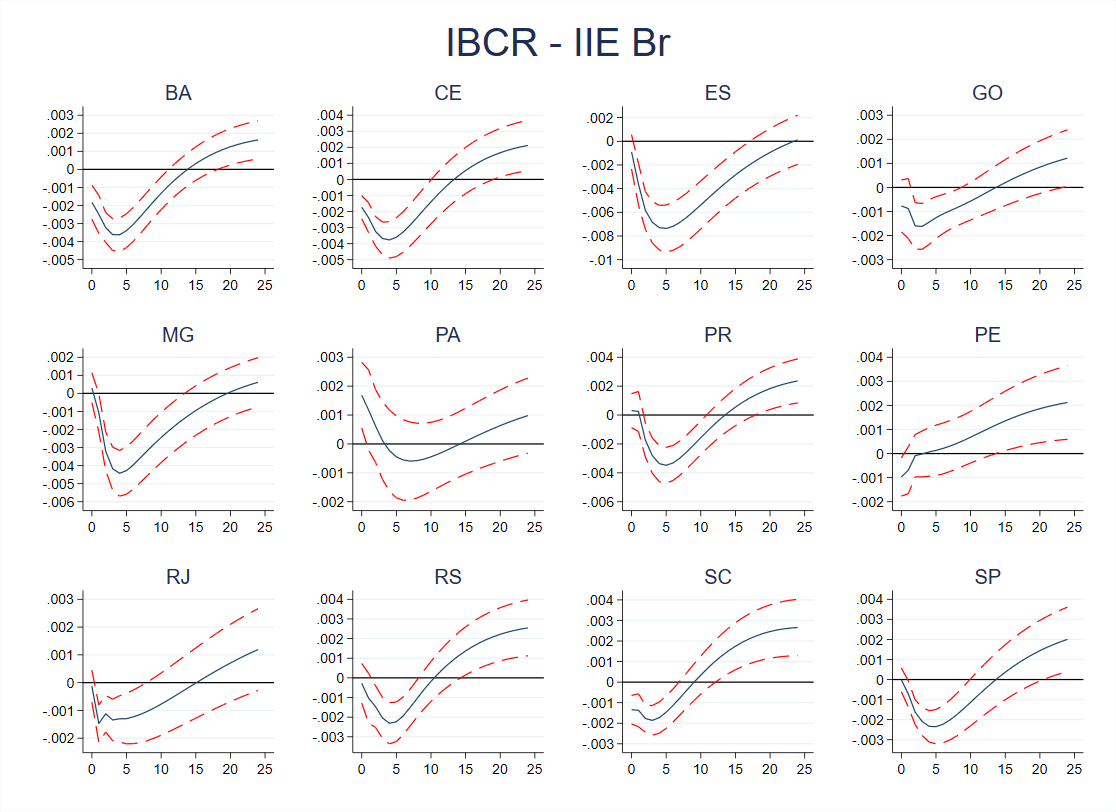
\includegraphics[width=1\linewidth]{Artigo/Fig/IRF/IRF_IIE_IBCR.png}
    \end{center}
    \label{fig:IRF_IIE_IBCR}
Fonte: Elaboração própria. \newline
Nota: Respostas estaduais após o choque de um desvio padrão na medida de incerteza. Os números do gráfico estão descritos em valores absolutos. A linha tracejada em vermelho representa o intervalo de confiança de 68\%.
\end{figure}

%\begin{figure}[htb!]
%    \caption{Respostas acumulada até o 12\textordmasculine\ período após um choque de 1\% do IIE-Br}
%    \label{fig:map_irf_IBCR_PIM_IIE}
%    \begin{center}
%    \subfigure[IBCR]{
%        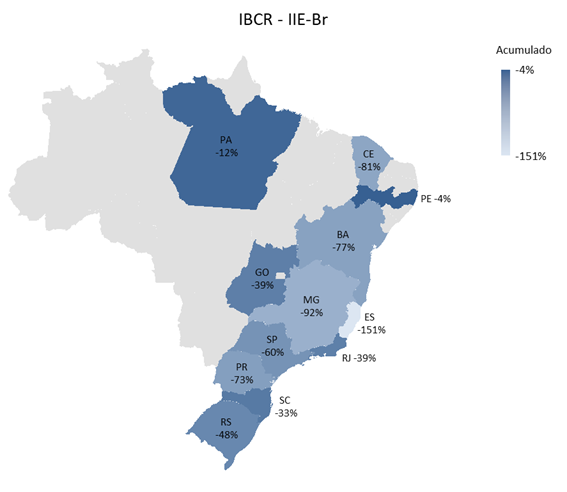
\includegraphics[width=0.45\linewidth]{Artigo/Fig/Maps/map_irf_IBCR_IIE.png}
%    }
%        \subfigure[PIM-PF]{
%        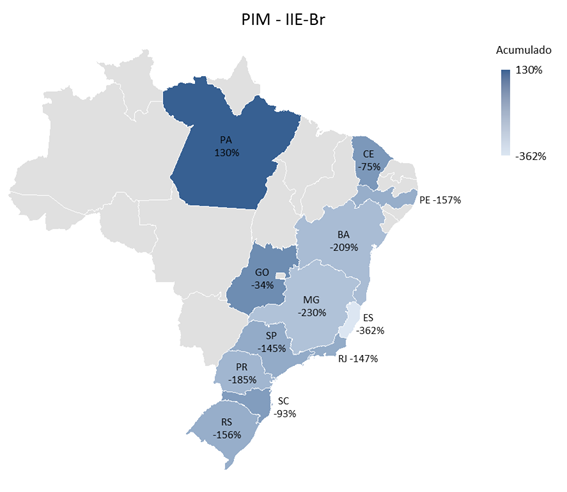
\includegraphics[width=0.45\linewidth]{Artigo/Fig/Maps/map_irf_PIM_IIE.png}
%    }
%    \end{center}
%Fonte: Elaboração própria. \newline
%Nota: Os números da função impulso resposta estão descritos em valores percentuais.
%\end{figure}

Conforme os resultados apresentados nas figuras \ref{fig:IRF_IIE_IBCR} e \ref{fig:IRF_IIE_PIM}, observa-se que o tamanho do impacto varia entre os estados. Em geral, há uma reação negativa mais profunda por parte da produção industrial.
Ademais, é evidente que a maior resposta das regiões para ambas as medidas de atividade econômica acontece entre o 3\textordmasculine\ e 5\textordmasculine\ mês após o choque, seguida de uma recuperação gradual também distinta em cada estado. Vale ressaltar ainda que o impacto acumulado se estende ao médio-longo prazo conforme a permanência de efeitos negativos acumulados até o 24\textordmasculine\ período.
\par

\begin{figure}[htb!]
    \caption{Respostas da PIM-PF após um choque da medida de incerteza IIE-Br}
    \begin{center}
        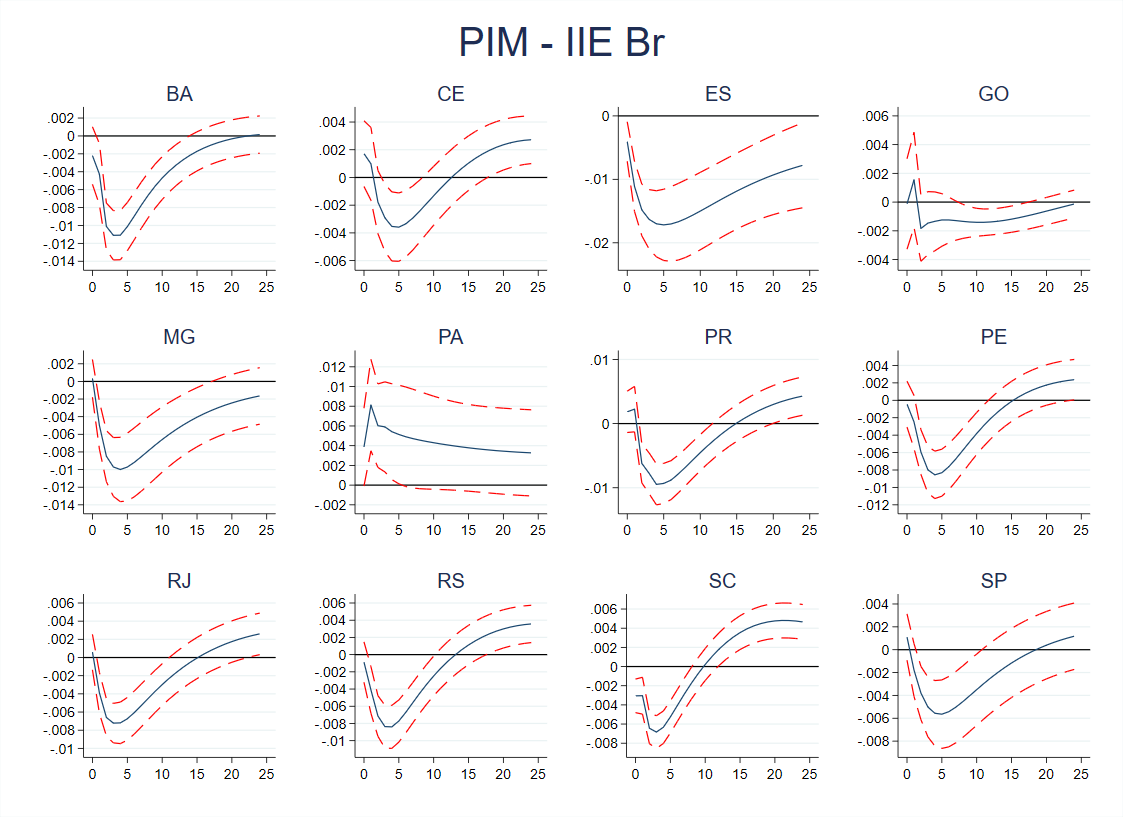
\includegraphics[width=1\linewidth]{Artigo/Fig/IRF/IRF_IIE_PIM.png}
    \end{center}
    \label{fig:IRF_IIE_PIM}
Fonte: Elaboração própria. \newline
Nota: Respostas estaduais após o choque de um desvio padrão na medida de incerteza. Os números do gráfico estão descritos em valores absolutos. A linha tracejada em vermelho representa o intervalo de confiança de 68\%.
\end{figure}

Em particular, os estados de \gls{GO}, \gls{PA} e \gls{PE} chamam atenção quanto à sua dinâmica de reação ao choque. Por exemplo, a resposta da produção industrial de \gls{GO} tem um impacto inicial positivo, o que difere do \gls{IBCR}, pois apresenta queda já no primeiro momento. Para o estado do \gls{PA}, o choque de incerteza é totalmente benéfico para a produção industrial, enquanto a atividade econômica agregada possui um impacto positivo inicial, um breve vale e retomada da atividade. Já no estado de \gls{PE}, ambas medidas de atividade econômica apresentam quedas, porém a recuperação da produção industrial é muito mais lenta quanto comparada a \textit{proxy} do \gls{PIB}, o \gls{IBCR}. 
\par

A diferença entre as proporções das respostas das duas medidas de atividade econômica sugere que, como proxy do \gls{PIB}, o \gls{IBCR} captura características de outros setores, não industriais, que mitigam ou até se beneficiam do choque de incerteza.

\subsubsection{Choque de incerteza: EPU}

\begin{figure}[htb!]
    \caption{Respostas do IBCR após um choque da medida de incerteza EPU}
    \begin{center}
        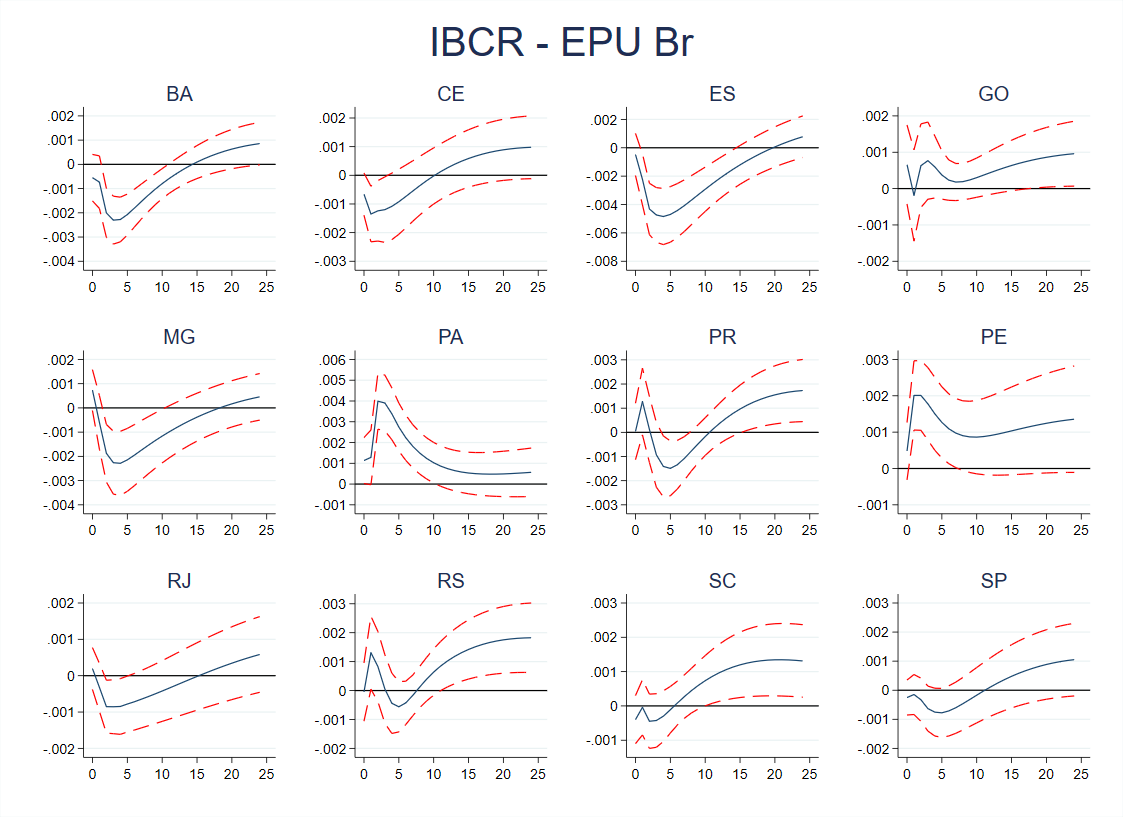
\includegraphics[width=1\linewidth]{Artigo/Fig/IRF/IRF_EPU_IBCR.png}
    \end{center}
    \label{fig:IRF_EPU_IBCR}
Fonte: Elaboração própria. \newline
Nota: Respostas estaduais após o choque de um desvio padrão na medida de incerteza. Os números do gráfico estão descritos em valores absolutos. A linha tracejada em vermelho representa o intervalo de confiança de 68\%.
\end{figure}

Considerando um choque de incerteza com a medida \gls{EPU}, de forma similar à medida \gls{IIE-Br}, os estados reagem de forma heterogênea e a produção industrial é mais impactada do que o \gls{IBCR}, além do maior efeito ser em geral no 3\textordmasculine\ e 4\textordmasculine\ mês após o choque. Porém, a proporção da reação ao choque com \gls{EPU} é um pouco menor, e isto sugere que as expectativas de mercado consideradas na medida \gls{IIE-Br} possuem uma maior influência sobre a atividade no geral. No caso do \gls{EPU}, a recuperação de médio-longo prazo é um pouco mais rápida quando comparada ao choque com \gls{IIE-Br}.
\par 
\begin{figure}[htb!]
    \caption{Respostas da PIM-PF após um choque da medida de incerteza EPU}
    \begin{center}
        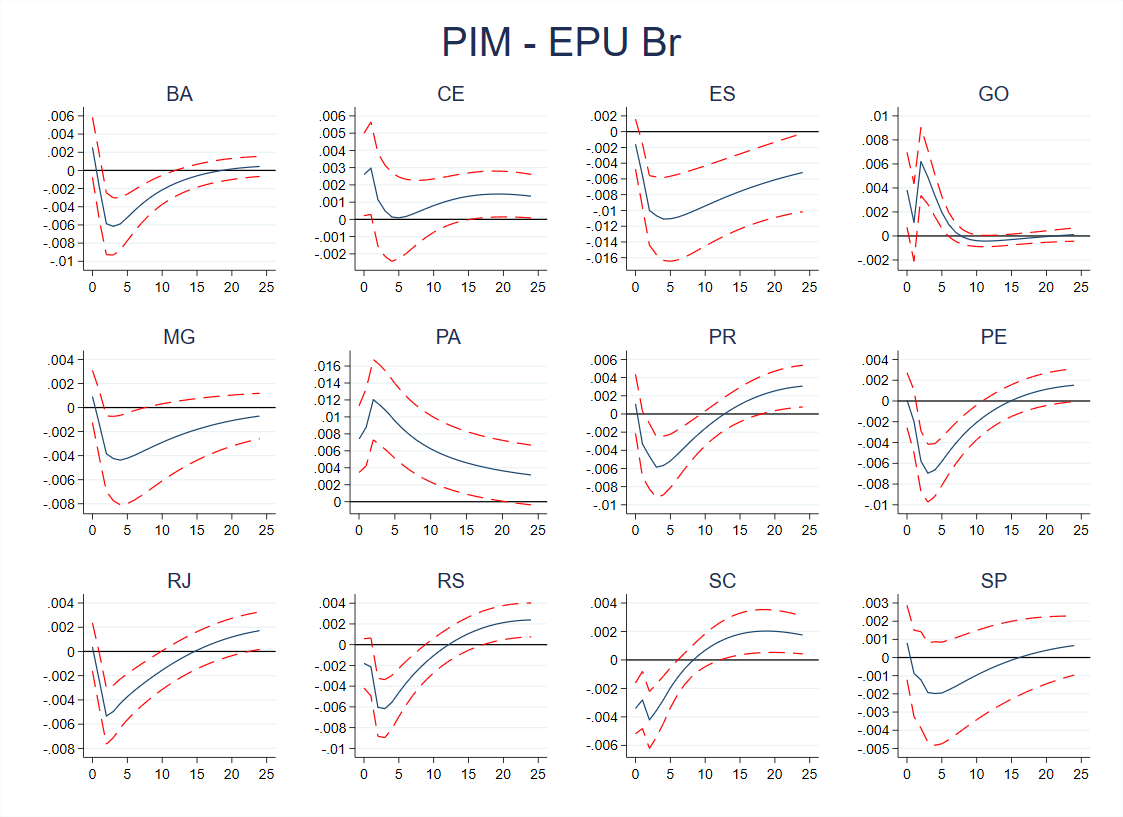
\includegraphics[width=1\linewidth]{Artigo/Fig/IRF/IRF_EPU_PIM.png}
    \end{center}
    \label{fig:IRF_EPU_PIM}
Fonte: Elaboração própria. \newline
Nota: Respostas estaduais após o choque de um desvio padrão na medida de incerteza. Os números do gráfico estão descritos em valores absolutos. A linha tracejada em vermelho representa o intervalo de confiança de 68\%.
\end{figure}

Dessa vez, os estados de \gls{CE}, \gls{GO} e \gls{PA} apresentam choque majoritariamente benéfico para a \gls{PIM-PF}, enquanto para o \gls{IBCR} isso apenas acontece para os estados de \gls{GO}, \gls{PA} e \gls{PE}. Particularmente, o estado de \gls{PE} apresenta um impacto positivo no \gls{IBCR}, porém negativo para a \gls{PIM-PF}. Este resultado sugere que as repostas podem ser heterogêneas entre as medidas de atividade econômica devido às características estruturais de cada local, e reforça a ideia da presença de concentração de setores não industriais que podem mitigar ou se beneficiar do choque. Ademais, vale ressaltar que as dinâmicas dos estados de \gls{PR} e \gls{RS} apresentam uma dinâmica inicial positiva, seguida de um breve vale e posteriormente uma recuperação quando observado o indicador \gls{IBCR}. Porém, no geral, a produção industrial apresenta impacto negativo mais profundo e duradouro.

\subsubsection{Choque de incerteza: GEPU}
\begin{figure}[htb!]
    \caption{Respostas do IBCR após um choque da medida de incerteza GEPU}
    \begin{center}
        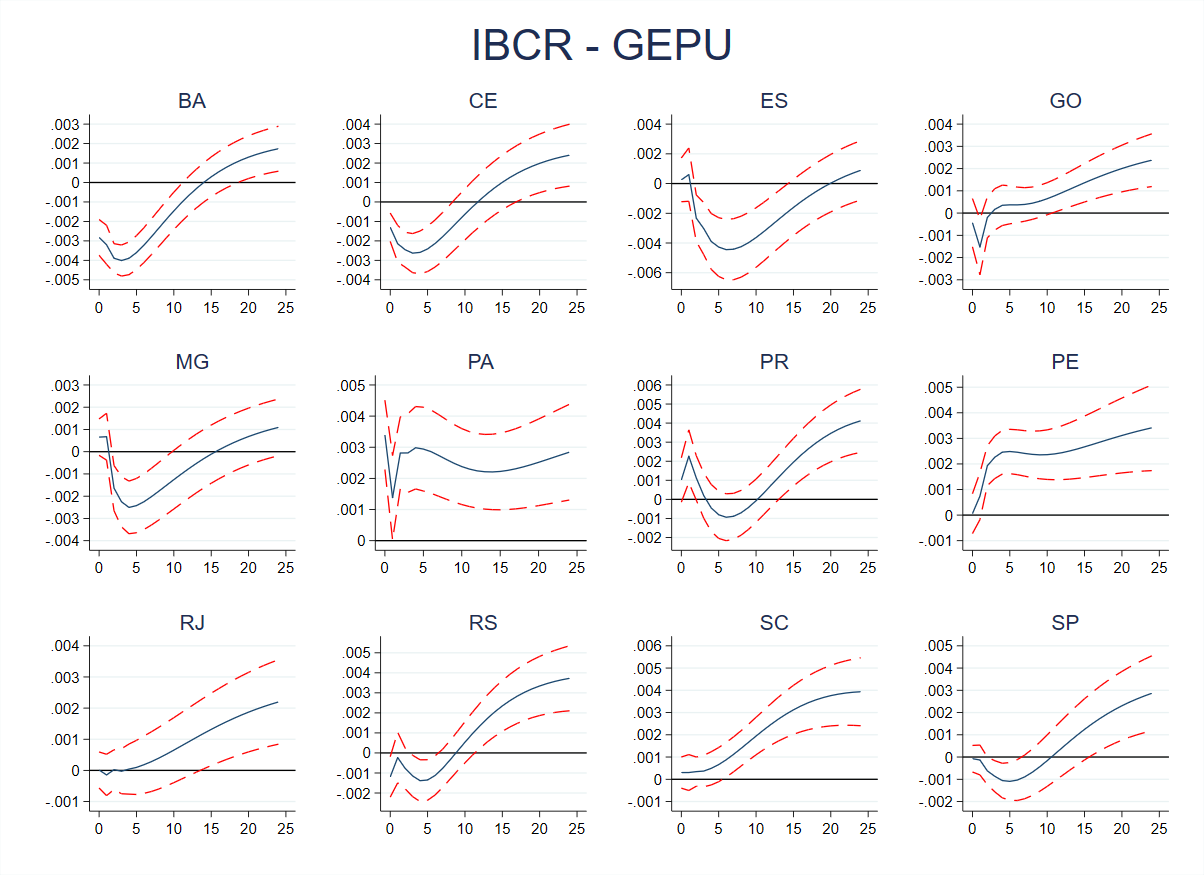
\includegraphics[width=1\linewidth]{Artigo/Fig/IRF/IRF_GEPU_IBCR.png}
    \end{center}
    \label{fig:IRF_GEPU_IBCR}
Fonte: Elaboração própria. \newline
Nota: Respostas estaduais após o choque de um desvio padrão na medida de incerteza. Os números do gráfico estão descritos em valores absolutos. A linha tracejada em vermelho representa o intervalo de confiança de 68\%.
\end{figure}

\begin{figure}[htb!]
    \caption{Respostas da PIM após um choque da medida de incerteza GEPU}
    \begin{center}
        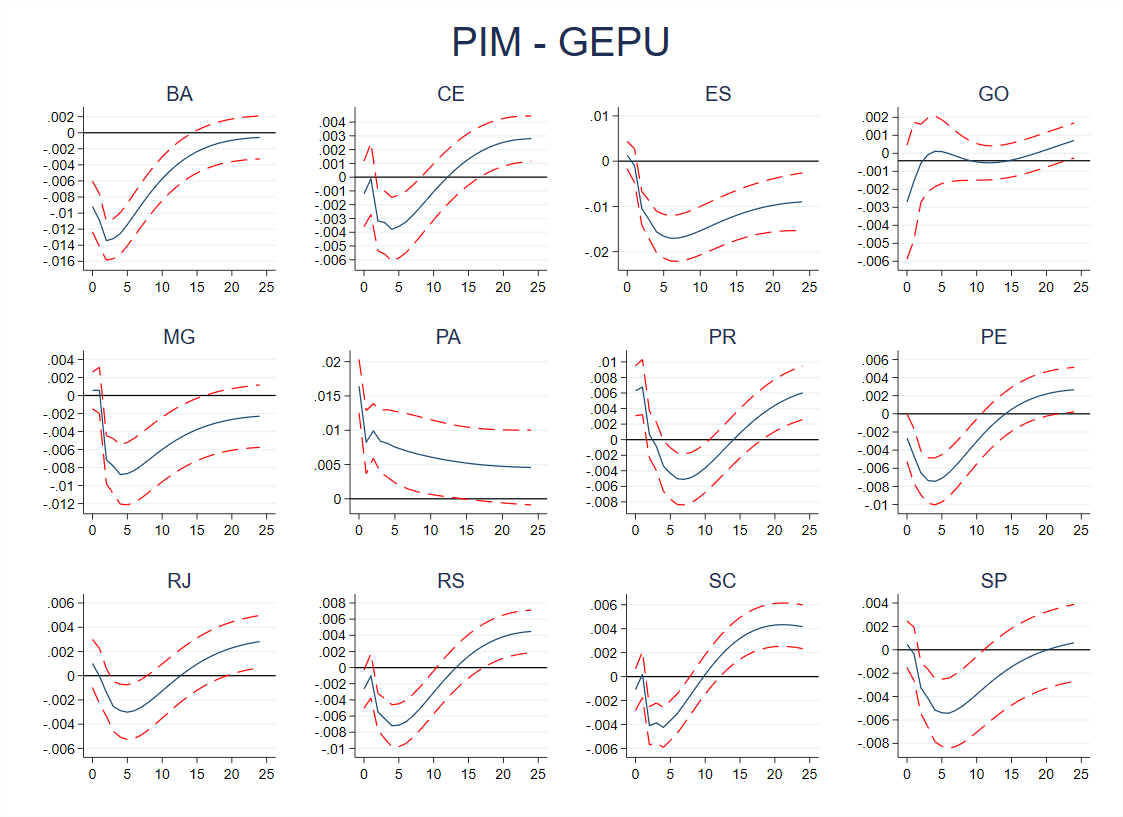
\includegraphics[width=1\linewidth]{Artigo/Fig/IRF/IRF_GEPU_PIM.png}
    \end{center}
    \label{fig:IRF_GEPU_PIM}
Fonte: Elaboração própria. \newline
Nota: Respostas estaduais após o choque de um desvio padrão na medida de incerteza. Os números do gráfico estão descritos em valores absolutos. A linha tracejada em vermelho representa o intervalo de confiança de 68\%.
\end{figure}

A partir da medida de incerteza \gls{GEPU}, observa-se que, em geral, o impacto de eventos externos induz uma resposta mais intensa quando comparada ao choque de notícias relacionadas à incerteza doméstica, \gls{EPU}, porém menor que o choque considerando as expectativas do mercado, \gls{IIE-Br}. Mais uma vez, a produção industrial é o indicador de atividade mais impactado, com a maior reação entre o 3\textordmasculine\ e 7\textordmasculine\ mês após o choque. A recuperação de um choque externo é mais rápida quando comparada ao choque de incerteza considerando expectativas e \gls{IIE-Br}, porém mais lenta quando considerada a incerteza doméstica \gls{EPU}. Isto indica que as expectativas de mercado possuem influência na persistência dos efeitos de um choque de incerteza. 
\par

Ao comparar o \gls{IBCR} a \gls{PIM-PF} após um choque de incerteza externa, os estados de \gls{PE}, \gls{RJ} e \gls{SC} apresentam as dinâmicas mais diferentes dentre os demais. Ao considerar o \gls{IBCR}, tais regiões apresentam uma reação majoritariamente positiva, enquanto a produção industrial sinaliza impacto negativo. E mais uma vez, o estado de \gls{PE} apresenta direções opostas entre as duas medidas de atividade econômica. 

\subsubsection{Robustez}

Para testar a robustez do modelo e das respostas obtidas, foram consideradas as seguintes variações descritas abaixo, cada uma aplicada separadamente, sendo os modelos:

\begin{enumerate}
    \item[1] Inclusão de tendência
    \item[2] Exclusão da série de emprego
    \item[3] Exclusão da série Ibovespa
    \item[4] Ordenação causal: Atividade, Emprego, Selic, Incerteza, Ibovespa
    \item[5] Ordenação causal: Incerteza, Atividade, Emprego, Selic, Ibovespa
    \item[6] Ordenação causal: Atividade, Emprego, Selic, Ibovespa, Incerteza
\end{enumerate}
Em geral, os resultados apresentam ser robustos, porém com algum grau de ressalva para certos modelos, estados e medidas de incerteza. Essa ressalva se baseia na comparação do modelo base considerando as diferenças de: intensidade do choque, formato da dinâmica de reação e taxa de recuperação da atividade econômica. Os gráficos do exercício de robustez podem ser consultados no apêndice \ref{section: Robustness}.

\subsubsection{Heterogeneidade das respostas estaduais}
\begin{table}[htb!]
\caption{Resultados da regressão \textit{cross-section}}
\label{table:cross_section_results}
\vspace{0.25cm}
\small
\begin{center}
\begin{tabular}{l c c c c c c
    %>{\centering\arraybackslash}m{0.5cm}
    %>{\centering\arraybackslash}m{1.5cm}
    %>{\centering\arraybackslash}m{1.25cm}
    %>{\centering\arraybackslash}m{1.5cm}
    %>{\centering\arraybackslash}m{1.25cm}
    %>{\centering\arraybackslash}m{2.25cm}
    %>{\centering\arraybackslash}m{2.25cm}
    %>{\centering\arraybackslash}m{2.25cm}
    }
  \hline
& Modelo 1 & Modelo 2 & Modelo 3 \\
  \hline
Agropecuária & 0.7310** & 0.4899 & 0.8976** \\
 & (0.1712) & (0.3084) & (0.1334) \\
Construção Civil & -1.7154 & -1.9447 & -0.5677 \\
 & (0.9082) & (0.9519) & (0.4271) \\
Indústria Extrativa & 0.4443* & 0.1432 & 0.5295* \\
 & (0.1875) & (0.3709) & (0.1481) \\
Indústria de Transformação & 1.0971** & 1.2331** & 1.2432*** \\
 & (0.3234) & (0.3579) & (0.1212) \\
Serviços Financeiros & 1.6235** & 1.5805** & 1.5479*** \\
 & (0.4090) & (0.4170) & (0.1414) \\
Serviços Públicos & 1.5445** & 1.7362** & 1.3967** \\
 & (0.3436) & (0.4030) & (0.1529) \\
Orçamento Público & -0.4639** & -0.5687** & -0.2683* \\
 & (0.1221) & (0.1661) & (0.0830) \\
Grau de Abertura &  & 0.1024 & 0.0007 \\
 &  & (0.1084) & (0.0421) \\ 
Densidade Demográfica &  &  & 0.0001** \\
 &  &  & (0.0000) \\
Constante & -0.3303** & -0.3263** & -0.4338*** \\
 & (0.0976) & (0.0990) & (0.0400) \\
\hline
R2 Ajustado & 0.61 & 0.60 & 0.95 \\
Observações & 12 & 12 & 12 \\
\hline
\end{tabular}
\end{center}
Fonte: Elaboração própria. \newline
Nota: Estão presentes os coeficientes dos modelos com os respectivos erros padrões entre parênteses. Níveis de significância estão descritos como: *** p<0.01; ** p<0.05; e * p<0.10. Esta tabela considera a resposta acumulada até o 9\textordmasculine\ período, $IRF_{i}^{9}$, para a estimação.
\end{table}

Para compreensão do porquê os estados apresentam respostas heterogêneas, foram estimados 3 modelos \textit{cross-section} apresentados na Tabela \ref{table:cross_section_results} abaixo. O primeiro modelo inclui características setoriais relativas ao \gls{PIB} dos respectivos estados, inclusive o grau de orçamento empenhado sobre o \gls{PIB}. O segundo modelo adiciona o grau de abertura econômica, e o terceiro modelo inclui a densidade demográfica de cada região. A análise do sinal desses modelos são robustos sabendo que houve resultados similares ao estimar o modelo com a \gls{FIR} acumulada para o 3\textordmasculine\, 6\textordmasculine\, 12\textordmasculine\ e 24\textordmasculine\ período, com exceção apenas para 6\textordmasculine\ e 24 \textordmasculine\ onde o grau de abertura e industria extrativa, respectivamente, são negativos.
\par

Todas as versões estimadas sugerem que os setores de agropecuária, indústria extrativa, industria de transformação, serviços financeiros, serviços públicos, além do grau de abertura econômica e a densidade demográfica, apresentam uma relação positiva, mesmo para os estados que apresentam uma resposta negativa. Isto revela que estados com maior presença dessas características são menos impactados por esses setores, ou pelo menos, a presença destes setores ajudam a mitigar o impacto negativo. Por outro lado, regiões com maior grau de orçamento público e participação do setor de construção civil em relação \gls{PIB} são mais fortemente impactados de forma negativa, o que pode sugerir precaução quanto a capacidade de pagamento da dívida estadual e também quanto a realização de investimentos em bens físicos de grande porte.
\par

Alguns setores, como agropecuária, serviços financeiros, indústria extrativa e de transformação, apresentam direções opostas da literatura comumente apresentada para o caso dos \gls{EUA}. Diante desse resultado, vale considerar que as estruturas das regiões brasileiras e estadunidense são diferentes, além de tudo, há a limitação de dados para o caso brasileiro, que possui observações de apenas de 12 dos 26 estados.
\par

Em resumo, após um choque de incerteza, é notório um impacto majoritariamente negativo e com diferentes proporções entre os estados, independente das três medidas de incertezas selecionadas, \gls{IIE-Br}, \gls{EPU} e \gls{GEPU}. Esses resultados corroboram com a evidência apresentada na literatura, por exemplo, \citeonline{bloom2009impact}, \citeonline{bloom2014fluctuations},  \citeonline{costa2014incerteza}, \citeonline{barboza2018efeitos}, \citeonline{mumtaz2018does}, \citeonline{mumtaz2018stateimpact} e \citeonline{silva2024effects}.
Porém há exceção para algumas situações que possuem respostas predominantemente positivas a depender da medida de incerteza e da medida de atividade econômica, como por exemplo no caso dos estados do \gls{CE}, \gls{GO}, \gls{PA}, \gls{PE}, \gls{RJ} e \gls{SC}. 
\par

Os maiores impactos ocorrem com a medida de incerteza \gls{IIE-Br} e da \gls{PIM-PF}, entre o terceiro e quinto mês. Isto indica uma maior influência das expectativas do mercado financeiro sobre a atividade econômica, e maior reação da produção industrial quando comparada ao \gls{IBCR}. Já o choque externo, \gls{GEPU}, é mais significativo do que o choque interno \gls{EPU}, o que corrobora com a evidência de \citeonline{bloom2017observations} de que, países em desenvolvimento tendem a reagir um pouco mais a choques externos. Porém, essa reação é menos significante quando comparada ao \gls{IIE-Br} com expectativas do mercado.
\par

O modelo \ref{eq:model_2} de regressão \textit{cross-section}, explora a relação entre a resposta e aspectos estruturais dos estados. Os coeficientes positivos indicam que regiões com maior participação dessas características serão menos afetadas pela incerteza, ou seja, trazem benefícios. O contrário é recíproco: estados com maior participação de setores com o coeficiente negativo serão mais impactados negativamente pela incerteza, e, portanto, trazem certo prejuízo.
\par

Os resultados da regressão sugerem que há setores como agropecuária, financeiro, indústria extrativa e de transformação são benéficos para reduzir a incerteza na economia dos estados brasileiros, porém, esse achado difere da evidência apresentada por \citeonline{mumtaz2018stateimpact}, em relação a um choque de incerteza agregado sobre as regiões dos \gls{EUA}, onde o setor de agricultura e de transformação são inteiramente negativos.  
\par

Também é importante considerar a participação do governo na economia, dessa forma, quanto maior o percentual de serviços públicos relacionados a administração, defesa, saúde, educação e seguridade social em relação ao \gls{PIB}, maiores são os benefícios para mitigar a incerteza, porém, quanto maior o grau de orçamento do estado em relação ao próprio \gls{PIB}, maior o será o impacto negativo, o que corrobora com a análise realizada por \citeonline{silva2024effects} através de um estudo para o caso de um choque de incerteza advindo do mercado imobiliário nos \gls{EUA}.
\par

Por fim, as unidades federativas com maior grau de abertura e maior densidade demográfica são menos impactadas pela incerteza, no entanto, o trabalho de \citeonline{rocha2011estados} para o choque de política monetária nos estados brasileiros apresenta o efeito oposto para a densidade demográfica, o que indica reações diferentes também entre um choque política monetária e um choque de incerteza.
\par

Em suma, a primeira análise apresenta que os estados reagem de forma heterogênea, em geral, de forma negativa, com diferentes proporções, dinâmicas e medidas de incerteza e produção. Já a segunda análise compreende que esta heterogeneidade se dá devido a aspectos estruturais e econômicos das regiões, como concentração de setores específicos, grau de abertura e orçamento público.

\newpage
\section{Conclusão}
Este trabalho investigou os efeitos de choques de incerteza agregado sobre a dinâmica da atividade econômica dos estados brasileiros para verificar se há evidências de respostas heterogêneas entre as regiões e compreender a conexão entre estas respostas e a estrutura econômica das unidades federativas. Com o intuito de contribuir para o desenho de políticas macroeconômicas em resposta a choques de incerteza.
\par

As estimativas apresentadas através do modelo \gls{SVAR} demonstram que as unidades da federação brasileira respondem de forma heterogênea a choques de incerteza, tanto em termos de trajetória do choque quanto em proporção. Essas reações também variam conforme o tipo de incerteza e indicador de atividade econômica. Nota-se que a atividade econômica é mais afetada pela \textit{proxy} de incerteza que inclui expectativa do mercado financeiro, \gls{IIE-Br}, seguido pela medida de choque externos, \gls{GEPU}, e finalmente pela medida de choque domésticos por citações de jornal, \gls{EPU}. Entre os indicadores de atividade econômica, a produção industrial se demonstra muito mais responsiva ao choque de incerteza quando comparada a \textit{proxy} do \gls{PIB}, o \gls{IBCR}.
\par

Os resultados do modelo com corte transversal indicam que os choques estão relacionados à estrutura econômica dos estados. As unidades federativas com maior participação de setores como agropecuária, indústria extrativa, industria de transformação, serviços financeiros, serviços públicos e maior grau de abertura relativos ao \gls{PIB} do estado, são menos impactadas, no entanto, onde há maior participação de ramos de construção e alto orçamento público, são mais fortemente afetados.
\par

Esses resultados apontam que os estados reagem de forma heterogênea independente das diversas \textit{proxies} de incerteza e de atividade econômica. Essa diversidade de reações estão baseadas em características estruturais e econômicas dos estados, como concentração de certos setores, grau de abertura e orçamento público.
\include{Artigo/4_referencias}

\bibliographystyle{abntex2-alf}
\bibliography{Artigo/4_referencia}

\appendix
%\section{Appendix - Resultados} \label{section:Results}

%\subsection{IIE-Br}

%\begin{table}[htb!]
%\caption{Respostas do \gls{IBCR} ao choque de 1\% do \gls{IIE-Br}}
%\label{table:irf_IBCR_IIE}
%\vspace{0.25cm}
%\small
%\begin{tabular}{
%    >{\centering\arraybackslash}m{0.5cm}
%    >{\centering\arraybackslash}m{1.5cm}
%    >{\centering\arraybackslash}m{1.25cm}
%    >{\centering\arraybackslash}m{1.5cm}
%    >{\centering\arraybackslash}m{1.25cm}
%    >{\centering\arraybackslash}m{2.25cm}
%    >{\centering\arraybackslash}m{2.25cm}
%    >{\centering\arraybackslash}m{2.25cm}
%    }
%  \hline
% UF & \makecell{Resposta \\ Mínima} & \makecell{Mês da \\ Mínima} & \makecell{Resposta \\ Máxima} & \makecell{Mês da \\ Máxima} & \makecell{Resposta \\ Acumulada \\ Até o 3 \textordmasculine\ Mês} & \makecell{Resposta \\ Acumulada \\ Até o 12\textordmasculine\ Mês} & \makecell{Resposta \\ Acumulada \\ Até o 24\textordmasculine\ Mês} \\
%  \hline
%  
%\gls{BA} & -0.0896 & 5 & 0.0341 & 25 & -0.1873 & -0.7659 & -0.6343 \\ 
%\gls{CE} & -0.0939 & 5 & 0.0437 & 25 & -0.1813 & -0.8067 & -0.6137 \\     
%\gls{ES} & -0.1601 & 6 & -0.0031 & 25 & -0.2294 & -1.5132 & -2.1144 \\    
%\gls{GO} & -0.0436 & 4 & 0.0195 & 25 & -0.0853 & -0.3874 & -0.3775 \\    
%\gls{MG} & -0.1112 & 5 & 0.0114 & 25 & -0.1220 & -0.9237 & -1.1331 \\
%\gls{PA} & -0.0217 & 8 & 0.0229 & 1 & 0.0380 & -0.1200 & -0.1020 \\      
%\gls{PR} & -0.0927 & 6 & 0.0543 & 25 & -0.0920 & -0.7315 & -0.4800 \\     
%\gls{PE} & -0.0270 & 1 & 0.0433 & 25 & -0.0555 & -0.0429 & 0.3230 \\      
%\gls{RJ} & -0.0424 & 2 & 0.0204 & 25 & -0.0852 & -0.3899 & -0.4060 \\ 
%\gls{RS} & -0.0681 & 5 & 0.0582 & 25 & -0.0965 & -0.4821 & -0.0663 \\     
%\gls{SC} & -0.0495 & 4 & 0.0602 & 25 & -0.1194 & -0.3253 & 0.1908 \\      
%\gls{SP} & -0.0706 & 6 & 0.0473 & 25 & -0.0963 & -0.6009 & -0.4153 \\  
%
%   \hline
%\end{tabular}
%\vspace{0.25cm}
%\newline
%Fonte: Elaboração própria. \newline
%Nota: Os números da função impulso resposta estão descritos em valores absolutos.
%\end{table}

%\subsection{GEPU}

\section{Appendix - Robustez} \label{section: Robustness}

\subsection{IIE-BR}

\begin{figure}[htb!]
    \caption{Robustez - IBCR após um choque da medida de incerteza IIE-Br}
    \begin{center}
        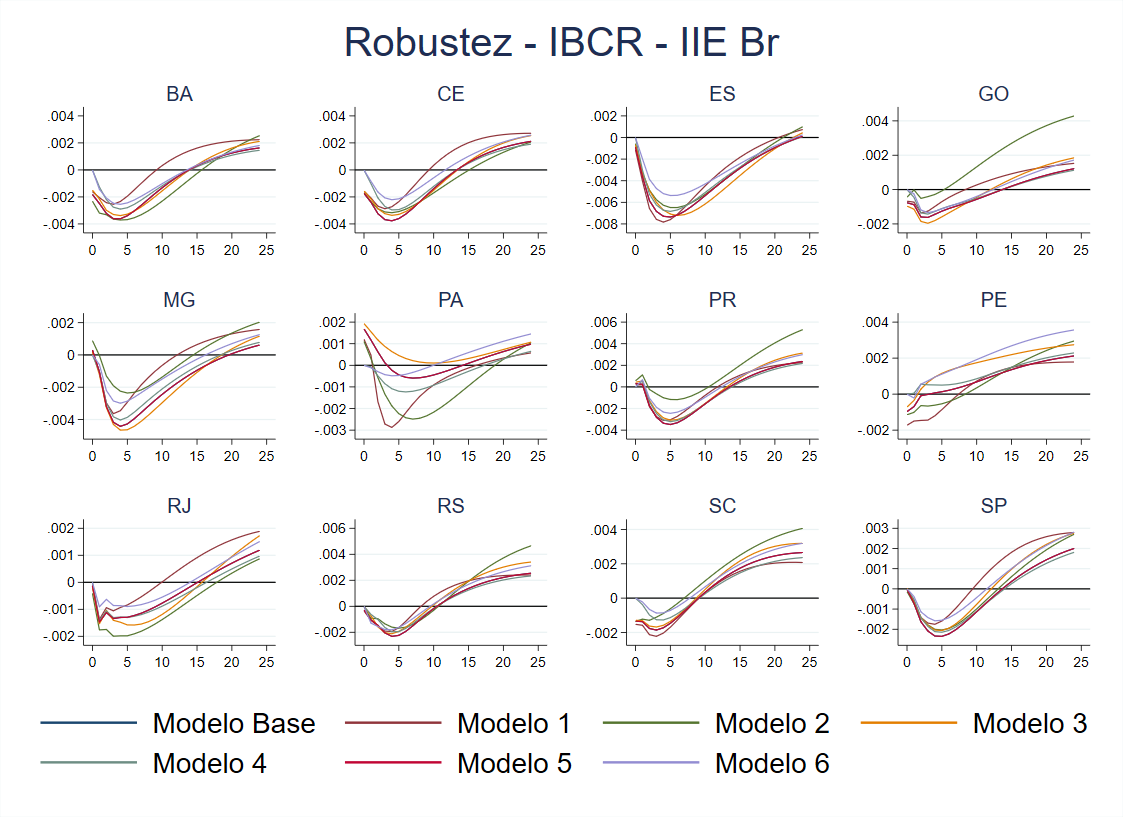
\includegraphics[width=1\linewidth]{Artigo/Fig/Robustness/IRF_IIE_IBCR_robustness.png}
    \end{center}
    \label{fig:IRF_IIE_IBCR_robustness}
Fonte: Elaboração própria. \newline
Nota: Respostas estaduais após o choque de um desvio padrão na medida de incerteza. Os números do gráfico estão descritos em valores absolutos. 
\end{figure}
\clearpage

\begin{figure}[htb!]
    \caption{Robustez - PIM após um choque da medida de incerteza IIE-Br}
    \begin{center}
        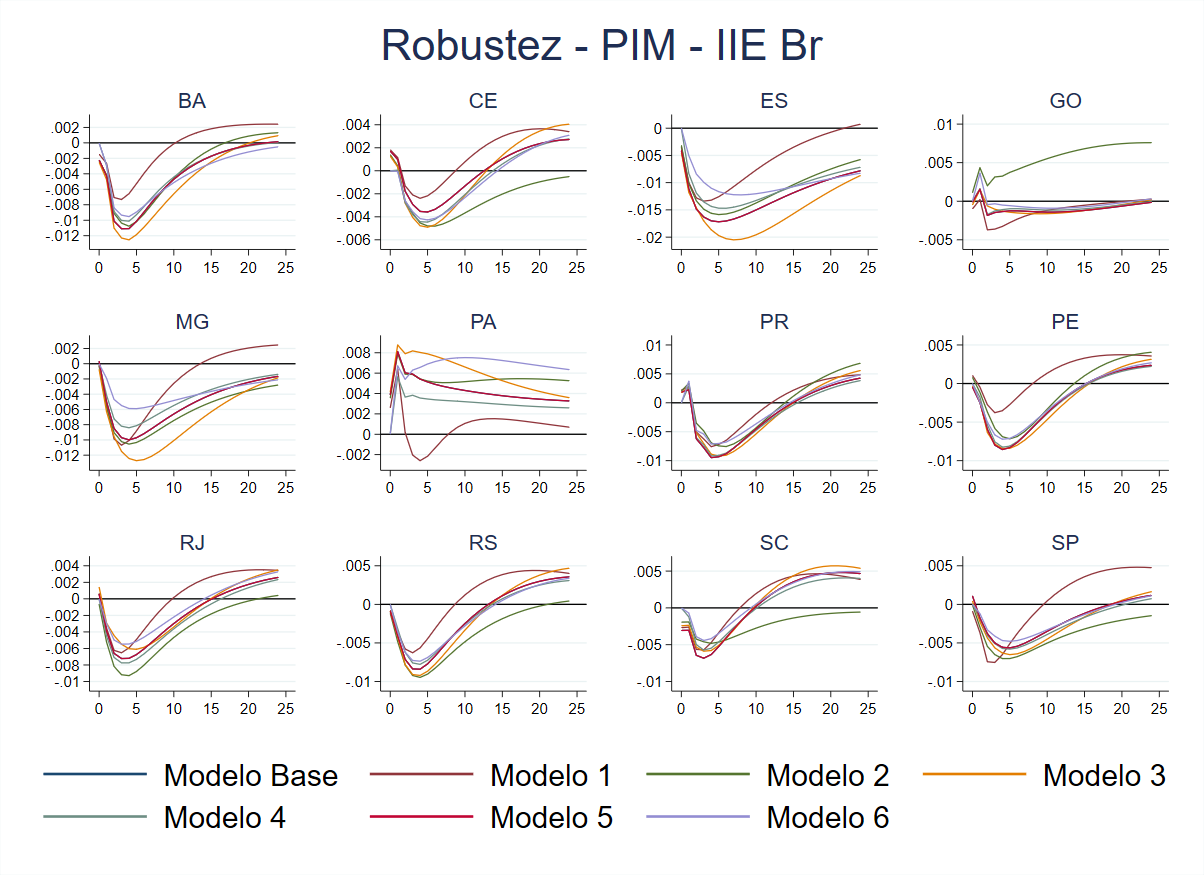
\includegraphics[width=1\linewidth]{Artigo/Fig/Robustness/IRF_IIE_PIM_robustness.png}
    \end{center}
    \label{fig:IRF_IIE_PIM_robustness}
Fonte: Elaboração própria. \newline
Nota: Respostas estaduais após o choque de um desvio padrão na medida de incerteza. Os números do gráfico estão descritos em valores absolutos.
\end{figure}
\clearpage

\subsection{EPU-BR}

\begin{figure}[htb!]
    \caption{Robustez - IBCR após um choque da medida de incerteza EPU-Br}
    \begin{center}
        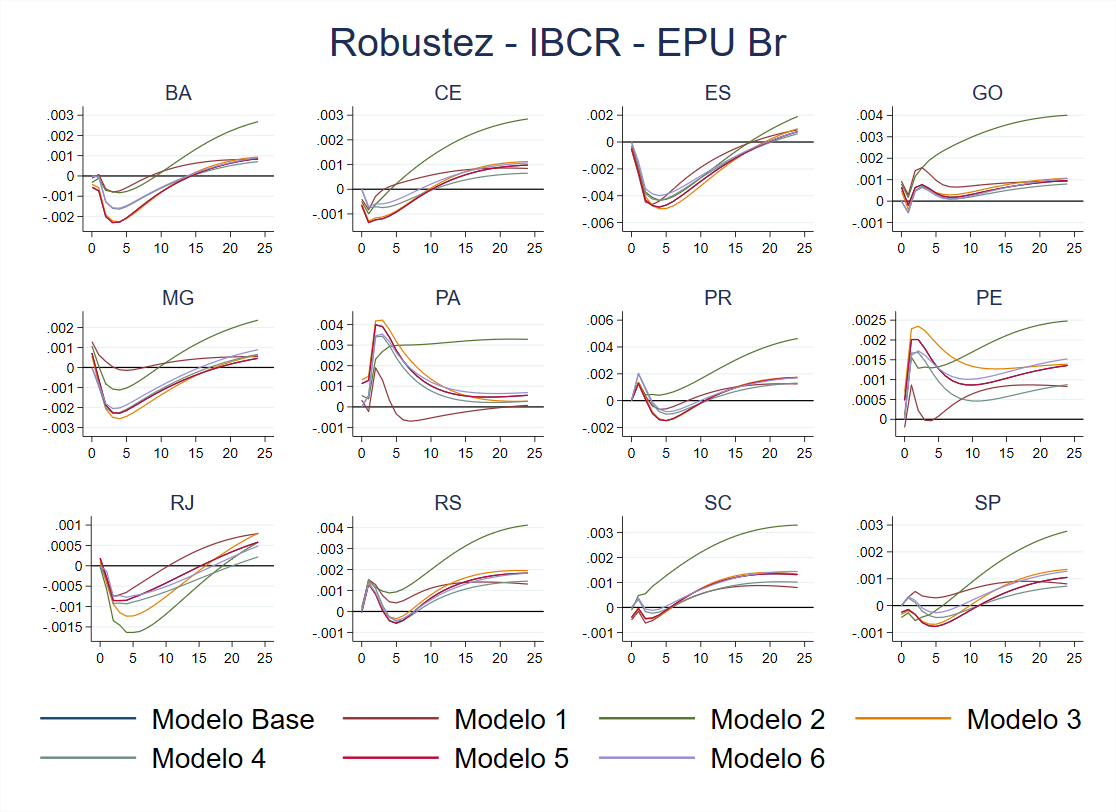
\includegraphics[width=1\linewidth]{Artigo/Fig/Robustness/IRF_EPU_IBCR_robustness.png}
    \end{center}
    \label{fig:IRF_EPU_IBCR_robustness}
Fonte: Elaboração própria. \newline
Nota: Os números da função impulso resposta estão descritos em valores absolutos.
\end{figure}
\clearpage

\begin{figure}[htb!]
    \caption{Robustez - PIM após um choque da medida de incerteza EPU-Br}
    \begin{center}
        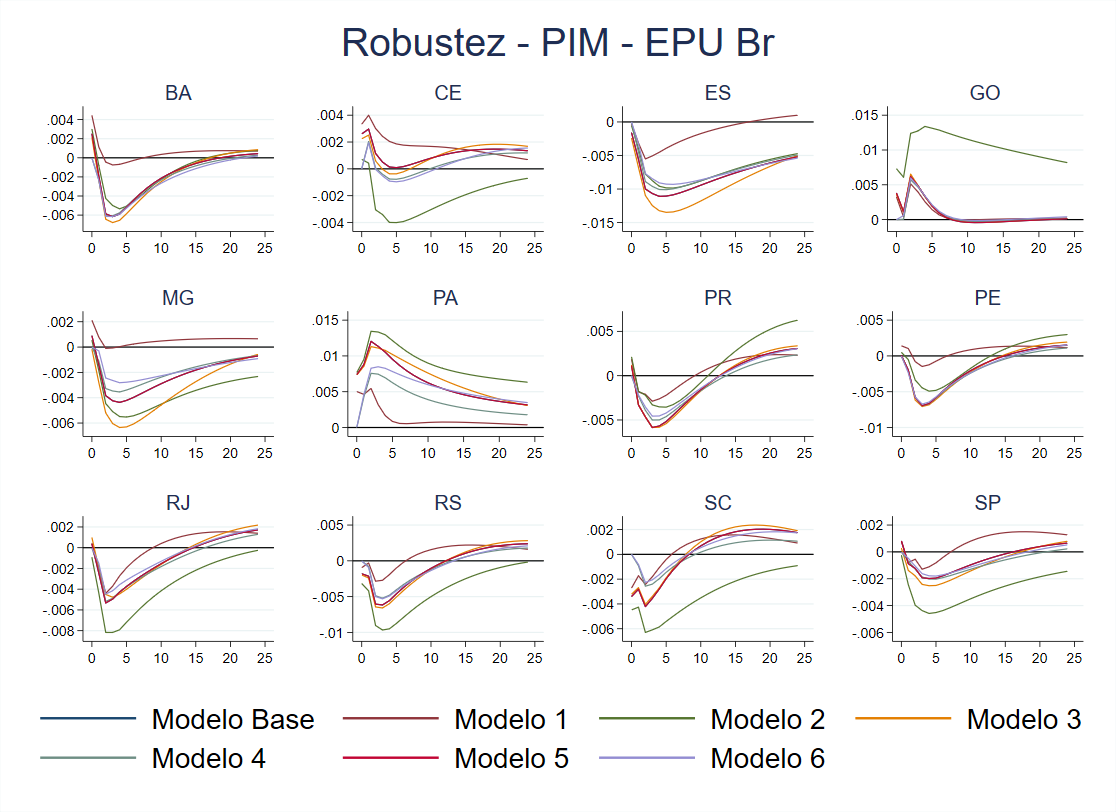
\includegraphics[width=1\linewidth]{Artigo/Fig/Robustness/IRF_EPU_PIM_robustness.png}
    \end{center}
    \label{fig:IRF_EPU_PIM_robustness}
Fonte: Elaboração própria. \newline
Nota: Os números da função impulso resposta estão descritos em valores absolutos.
\end{figure}
\clearpage

\subsection{GEPU}

\begin{figure}[htb!]
    \caption{Robustez - IBCR após um choque da medida de incerteza GEPU}
    \begin{center}
        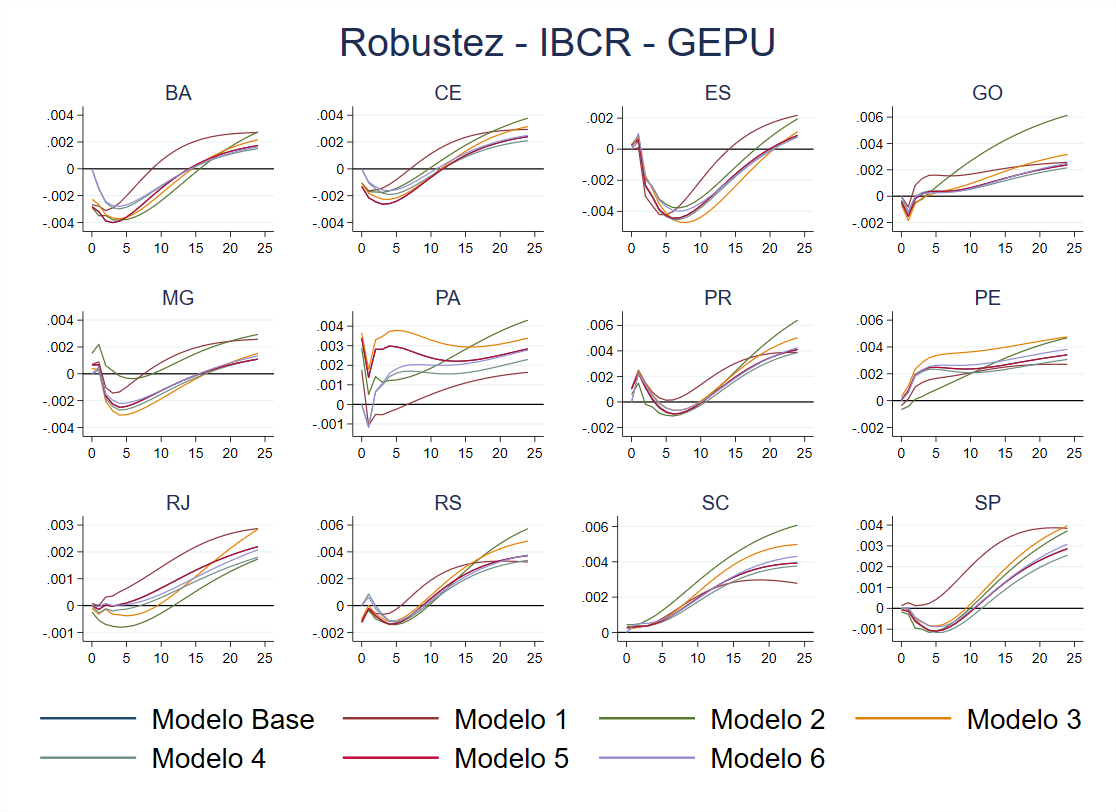
\includegraphics[width=1\linewidth]{Artigo/Fig/Robustness/IRF_GEPU_IBCR_robustness.png}
    \end{center}
    \label{fig:IRF_GEPU_IBCR_robustness}
Fonte: Elaboração própria. \newline
Nota: Os números da função impulso resposta estão descritos em valores absolutos.
\end{figure}
\clearpage

\begin{figure}[htb!]
    \caption{Robustez - PIM após um choque da medida de incerteza GEPU}
    \begin{center}
        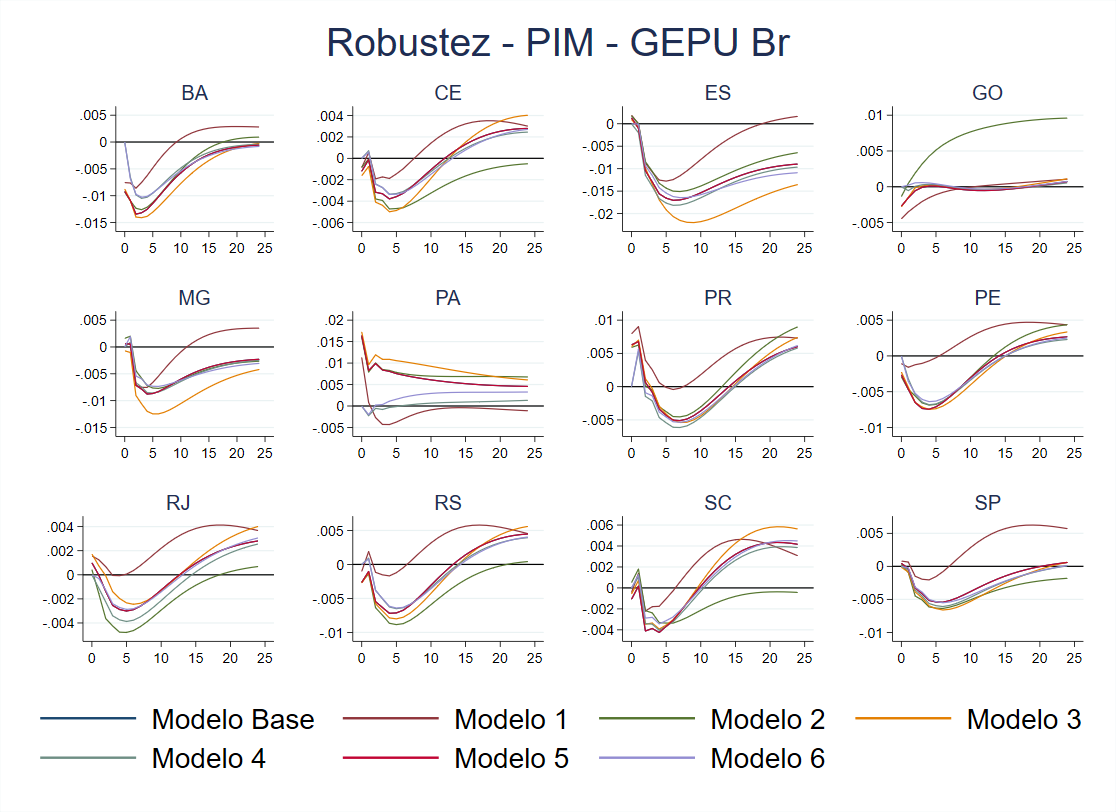
\includegraphics[width=1\linewidth]{Artigo/Fig/Robustness/IRF_GEPU_PIM_robustness.png}
    \end{center}
    \label{fig:IRF_GEPU_PIM_robustness}
Fonte: Elaboração própria. \newline
Nota: Os números da função impulso resposta estão descritos em valores absolutos.
\end{figure}
\clearpage

\section{Appendix - Cross-Section} \label{section:cross-section}

\begin{table}[htb!]
\caption{Descrição das variáveis utilizadas na regressão \textit{cross-section}}
\label{table:cross_section_labels}
\vspace{0.25cm}
\small
\begin{center}
\renewcommand{\arraystretch}{1.5}
\begin{tabular}{
    >{\raggedright\arraybackslash}m{3cm}
    |>{\raggedright\arraybackslash}m{7cm}
    |>{\centering\arraybackslash}m{2cm}
    |>{\centering\arraybackslash}m{3cm}
    %>{\centering\arraybackslash}m{1.25cm}
    %>{\centering\arraybackslash}m{2.25cm}
    %>{\centering\arraybackslash}m{2.25cm}
    %>{\centering\arraybackslash}m{2.25cm}
    }
  \hline
\textbf{Variável} & \textbf{Descrição} & \textbf{Ano(s)} & \textbf{Fonte} \\
\hline
PIB Estadual & PIB Estadual a preços de mercado (preços de 2010) & 2016 a 2019 & IPEADATA \\
\hline
\% Agropecuária & Produção agropecuária estadual dividido pelo PIB do respectivo estado & 2016 a 2019 & IPEADATA \\
\hline
\% Construção &  Produção da construção civil estadual dividido pelo PIB do respectivo estado & 2016 a 2019 & IPEADATA \\
\hline
\% Indústria Extrativa & Produção extrativa estadual dividido pelo PIB do respectivo estado & 2016 a 2019 & IPEADATA \\
\hline
\% Indústria de Transformação & Produção do setor de transformação estadual dividido pelo PIB do respectivo estado & 2016 a 2019 & IPEADATA \\
\hline
\% Serviços Financeiros & Produção de atividades financeiras, de seguros e serviços relacionados divididos pelo respectivo PIB estadual & 2016 a 2019 & IPEADATA \\
\hline
\% Serviços Públicos & Produção de serviços relacionados a administração, defesa, saúde e educação públicas e seguridade social divididos pelo respectivo PIB estadual & 2016 a 2019 & IPEADATA \\
\hline
\% Orçamento Público & Despesa corrente empenhada dividido pelo respectivo PIB estadual & 2016 a 2019 & IPEADATA \\
\hline
\% Grau de Abertura & Exportações menos importações divididos pelo respectivo PIB estadual & 2016 a 2019 & COMEXSTAT - GOV.BR \\
\hline
Densidade Demográfica & Habitante por quilômetro quadrado a nível das unidades federativas & 2022 & IBGE - Senso Demográfico 2022 - Tabela 4714 \\
\hline
\end{tabular}
\end{center}
Fonte: Elaboração própria. 
\end{table}

\end{document}
